% !TeX root = ..\main.tex
\section{Giao diện hệ thống}

\subsection{Giao diện chung}
\subsubsection{Đăng nhập}



\subsection{Giao diện người dùng}
\subsubsection{Đăng ký}



\subsubsection{Tạo lại mật khẩu}


\subsubsection{Header}


\subsubsection{Footer}



\subsubsection{Trang chủ}



\subsubsection{Giỏ hàng}


\subsubsection{Thanh toán}


\subsubsection{Giao diện quản lý đơn hàng}

\subsubsection{Giao diện chi tiết đơn hàng}

\subsubsection{Giao diện thông tin khách hàng}



\newpage
\subsection{Giao diện quản trị viên}
\subsubsection{Chung}
\subsubsubsection{Thay đổi mật khẩu}
\begin{figure}[!htp]
    \centering
    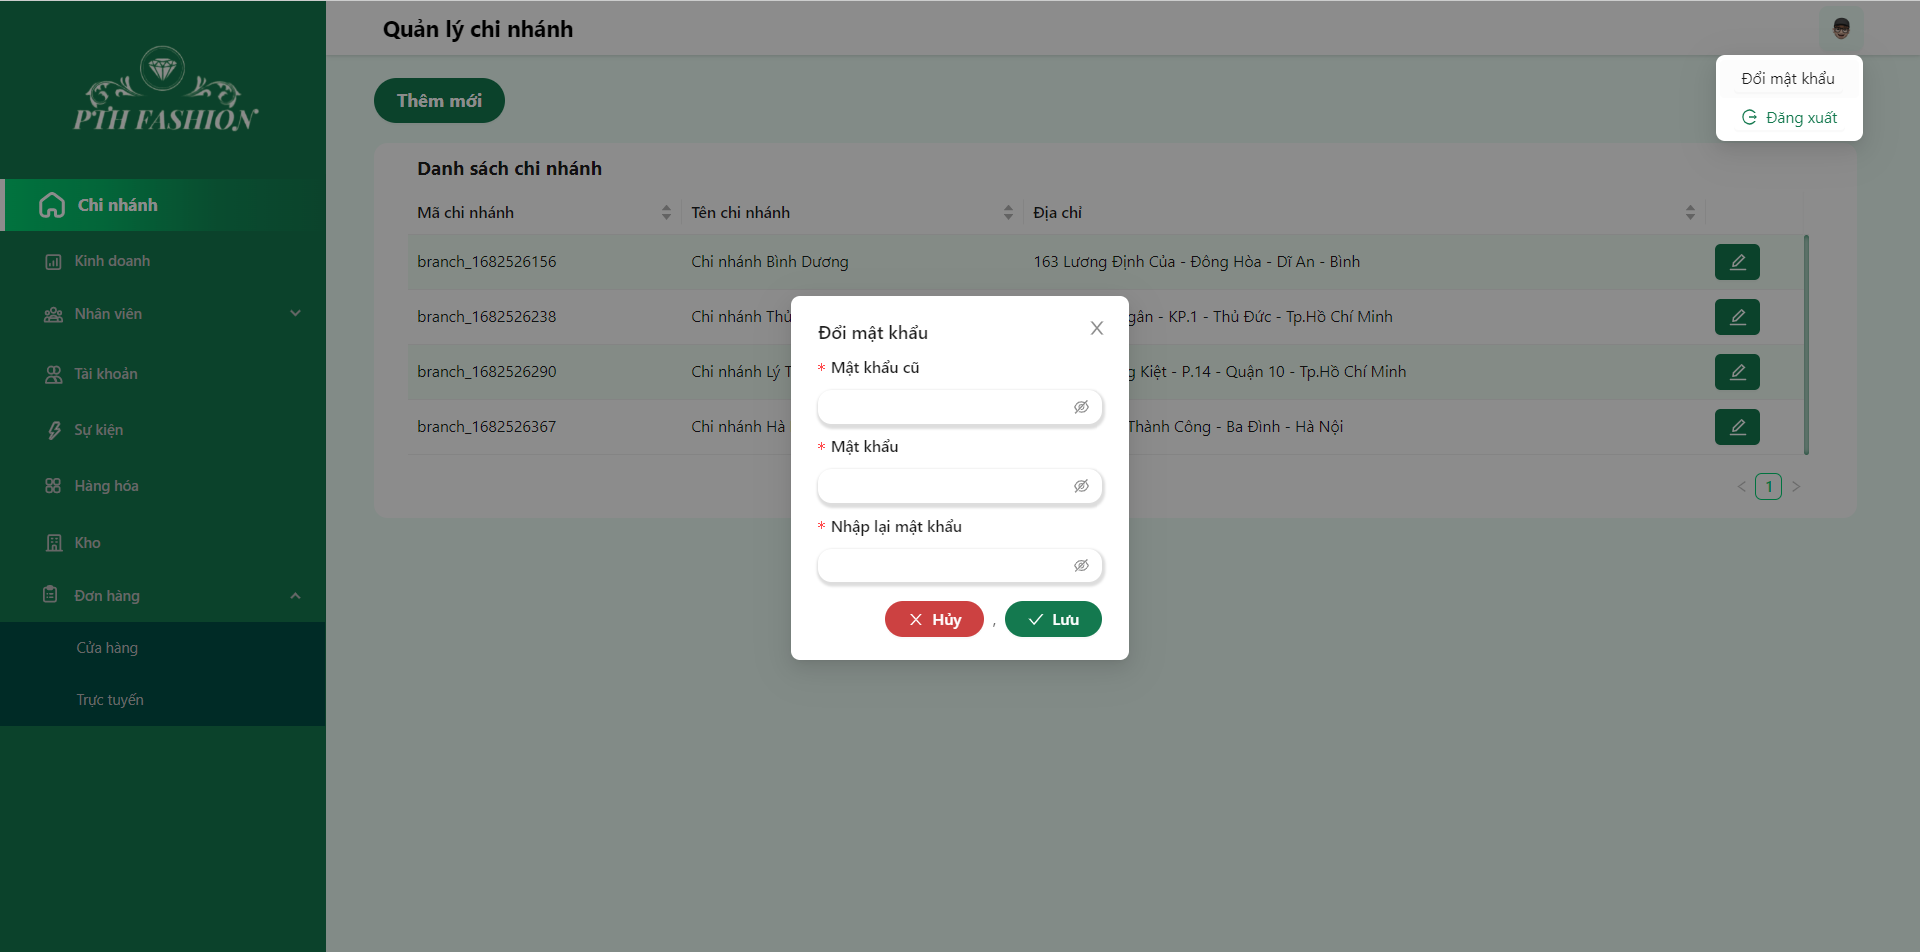
\includegraphics[width=12cm]{img/UI/admin_implement/changePassword.png}
    \label{20}
    \newline
    \caption{Giao diện thay đổi mật khẩu}
\end{figure}


\subsubsection{Quản lý chi nhánh}
\begin{figure}[!htp]
    \centering
    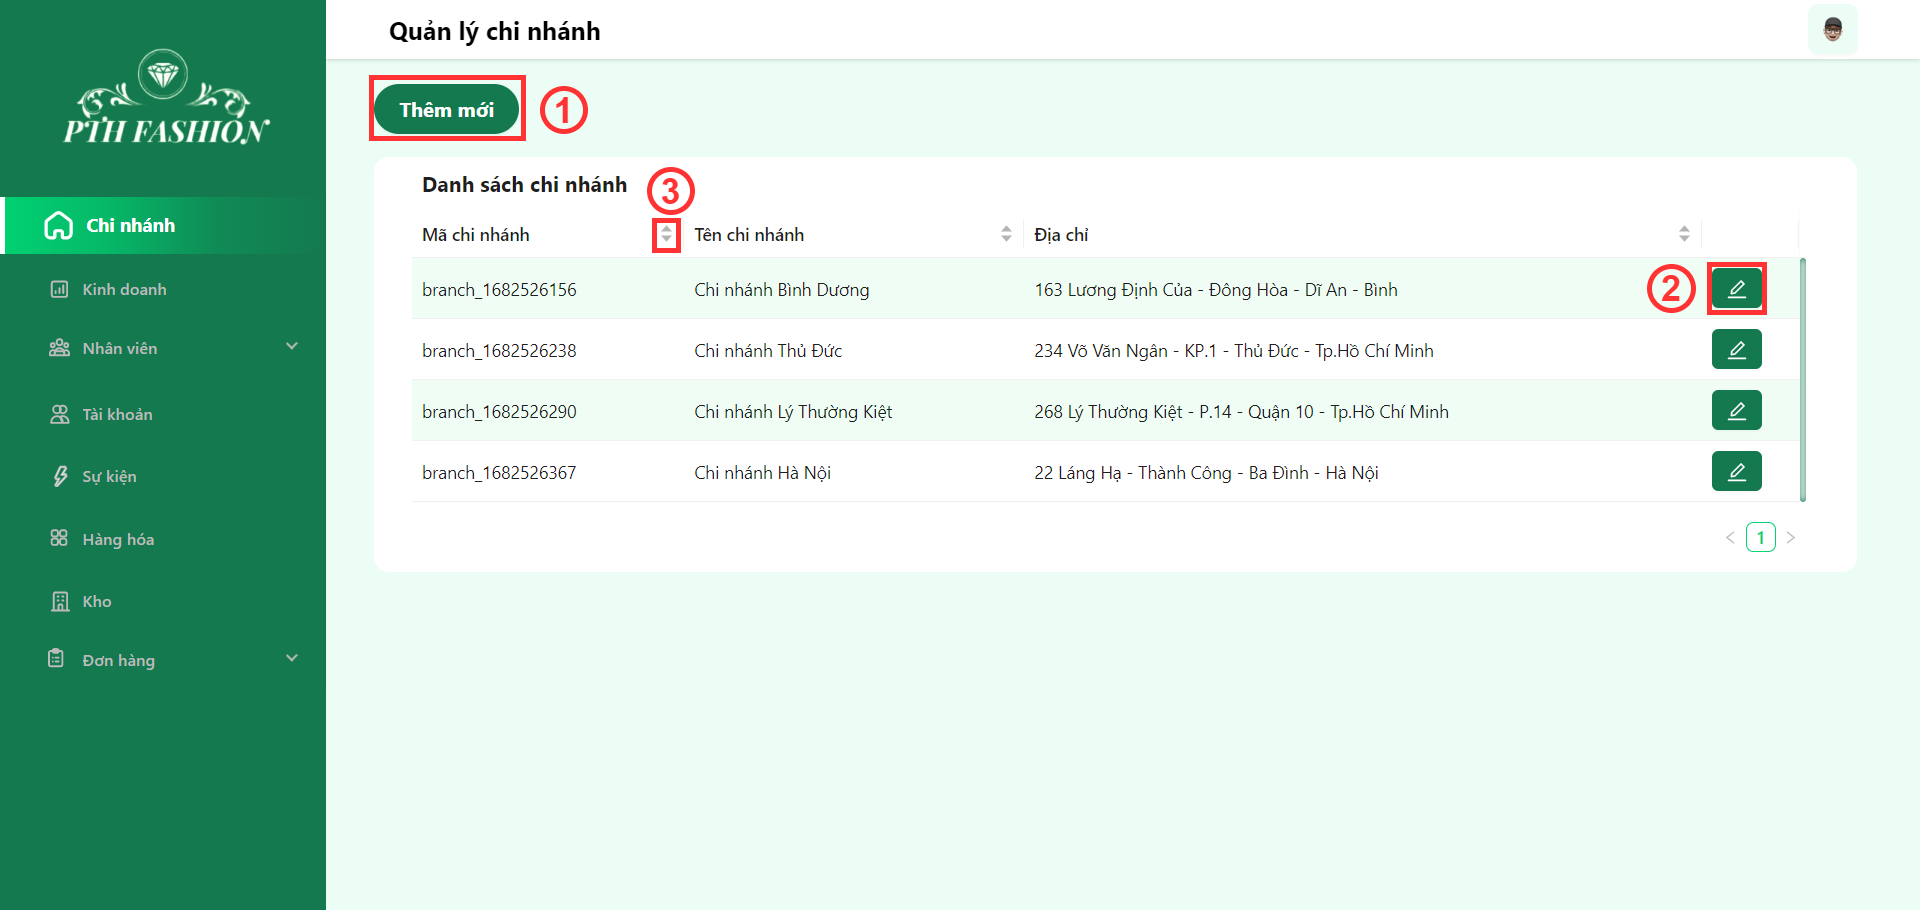
\includegraphics[width=12cm]{img/UI/admin_implement/branch.png}
    \newline
    \caption{Giao diện quản lý chi nhánh}
\end{figure}

\textbf{Mô tả:}
\begin{quote}
    \begin{enumerate}
        \item Chọn để thêm mới chi nhánh
        \item Chọn để chỉnh sửa thông tin chi nhánh
        \item Chọn sắp xếp danh sách chi nhánh theo id
    \end{enumerate}
    Hiển thị danh sách tất cả chi nhánh trong hệ thống. Tương tự cho các tính năng quản lý khác.
\end{quote}

\subsubsubsection{Thông tin chi tiết chi nhánh}
\begin{figure}[!htp]
    \centering
    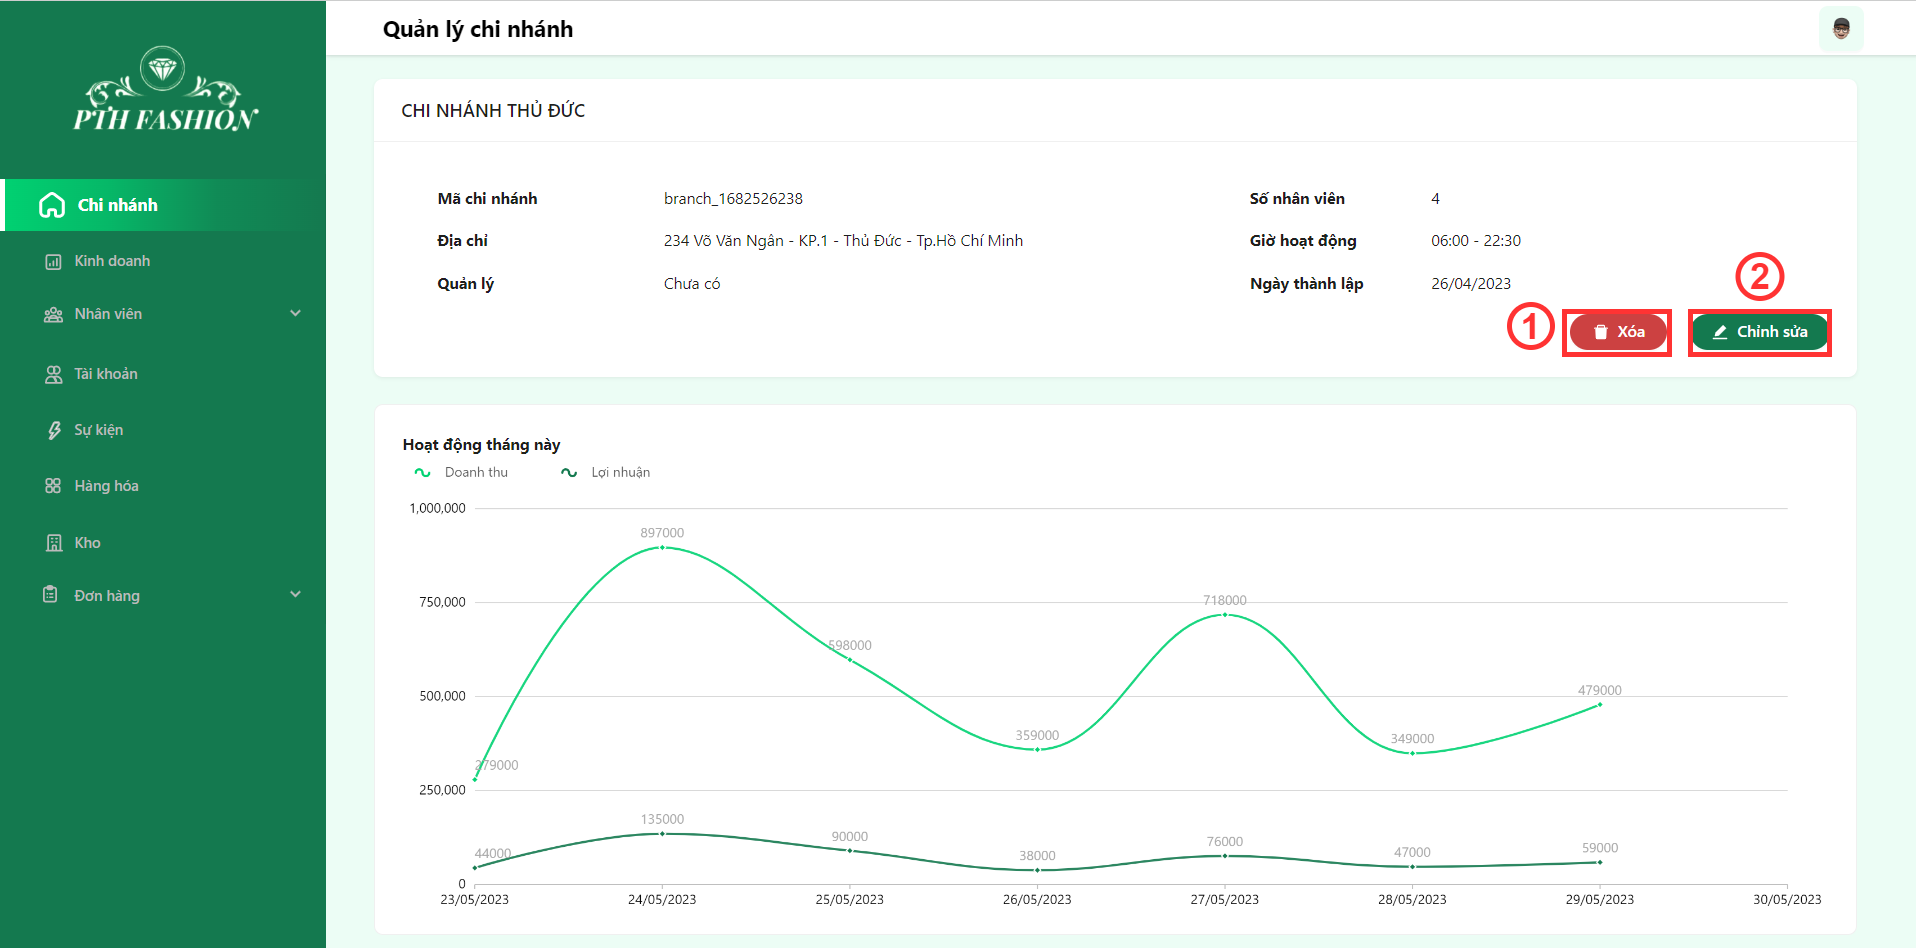
\includegraphics[width=12cm]{img/UI/admin_implement/branchDetail.png}
    \newline
    \caption{Giao diện thông tin chi tiết chi nhánh}
\end{figure}
\textbf{Mô tả:}
\begin{quote}
    \begin{enumerate}
        \item Chọn để xóa chi nhánh
        \item Chọn để hiển thị form "chỉnh sửa chi nhánh"
    \end{enumerate}
    Hiển thị danh sách thông tin chi tiết của chi nhánh. Tương tự cho các tính năng quản lý khác
\end{quote}


\subsubsubsection{Thêm chỉnh sửa chi nhánh}
\begin{figure}[!htp]
    \centering
    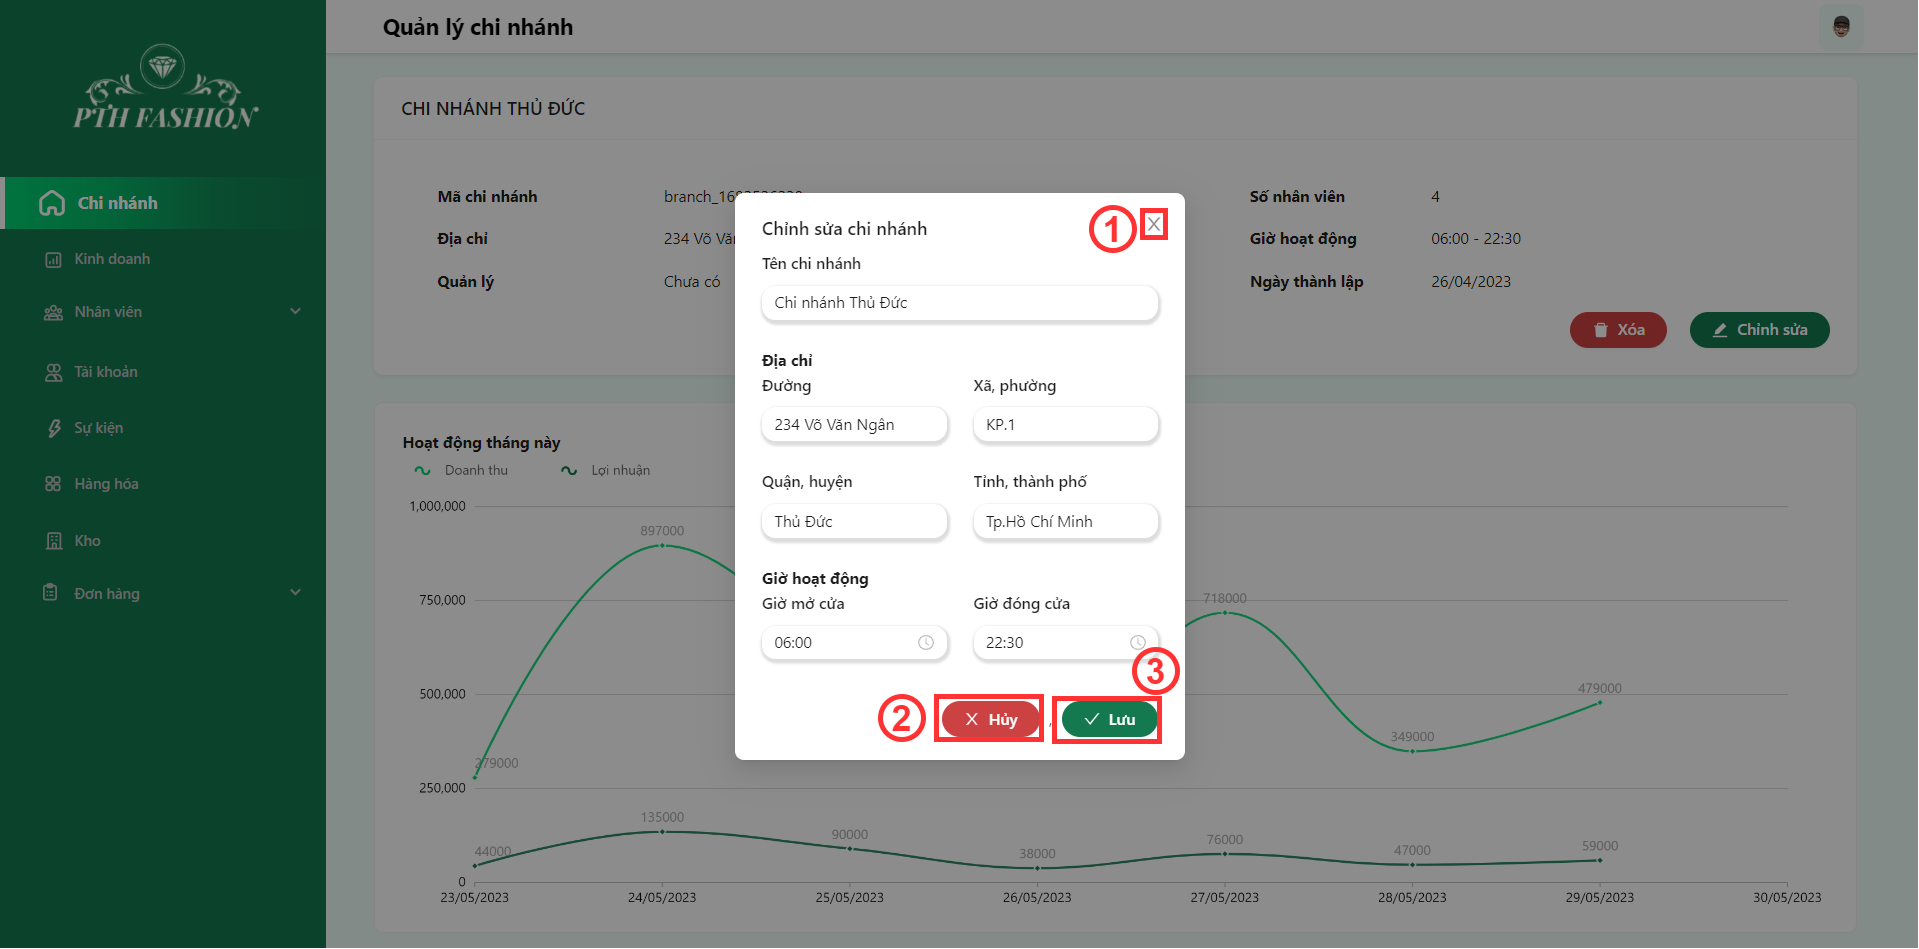
\includegraphics[width=12cm]{img/UI/admin_implement/branchEdit.png}
    \newline
    \caption{Giao diện form thêm mới, chỉnh sửa chi nhánh}
\end{figure}
\textbf{Mô tả:}
\begin{quote}
    \begin{enumerate}
        \item Chọn để hủy thay đổi
        \item Chọn để hủy thay đổi
        \item Chọn để lưu thay đổi
    \end{enumerate}
    Nhập các thông tin để thêm mới hoặc chỉnh sửa chi nhánh. Tương tự cho các tính năng quản lý khác
\end{quote}

\newpage

\subsubsection{Quản lý hoạt động kinh doanh}
\begin{figure}[!htp]
    \centering
    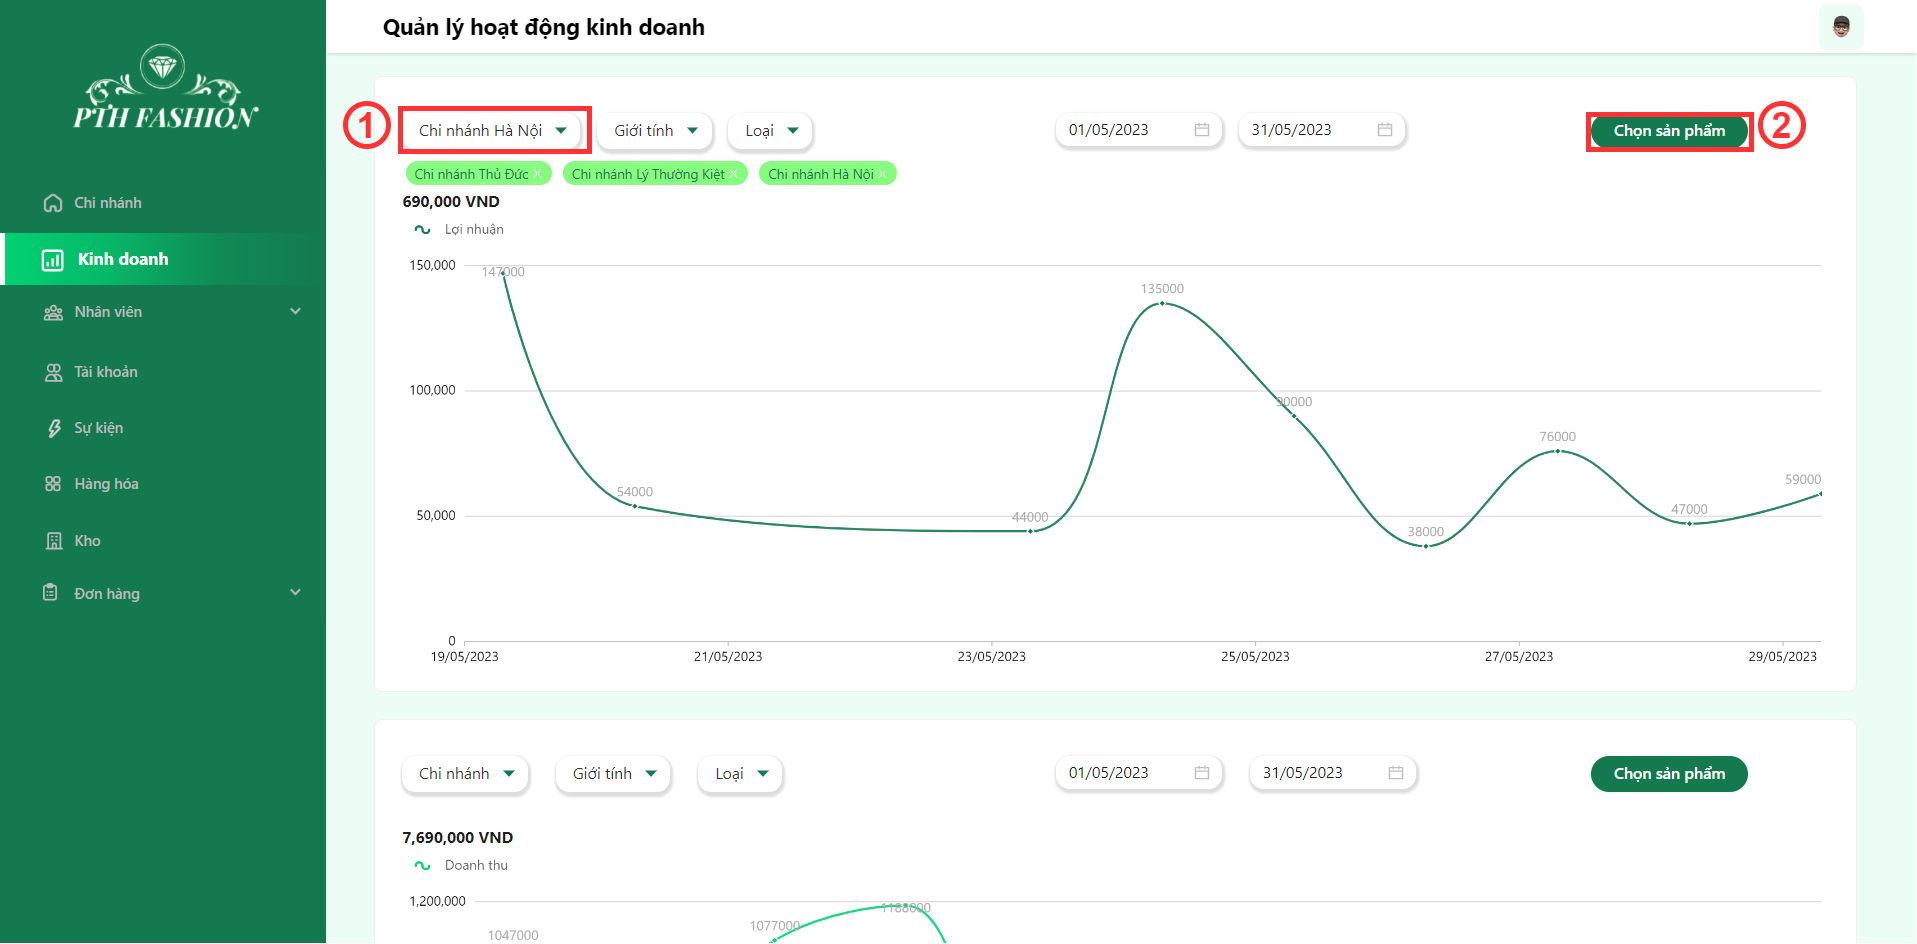
\includegraphics[width=12cm]{img/UI/admin_implement/statistic.png}
    \newline
    \caption{Giao diện quản lý hoạt động kinh doanh}
\end{figure}
\textbf{Mô tả:}
\begin{quote}
    \begin{enumerate}
        \item Chọn để lọc thống kê theo chi nhánh, tương tự với các tính năng lọc còn lại
        \item Chọn một sản phẩm để thống kê
    \end{enumerate}
\end{quote}

\newpage


\subsubsection{Quản lý nhân viên}
\begin{figure}[!htp]
    \centering
    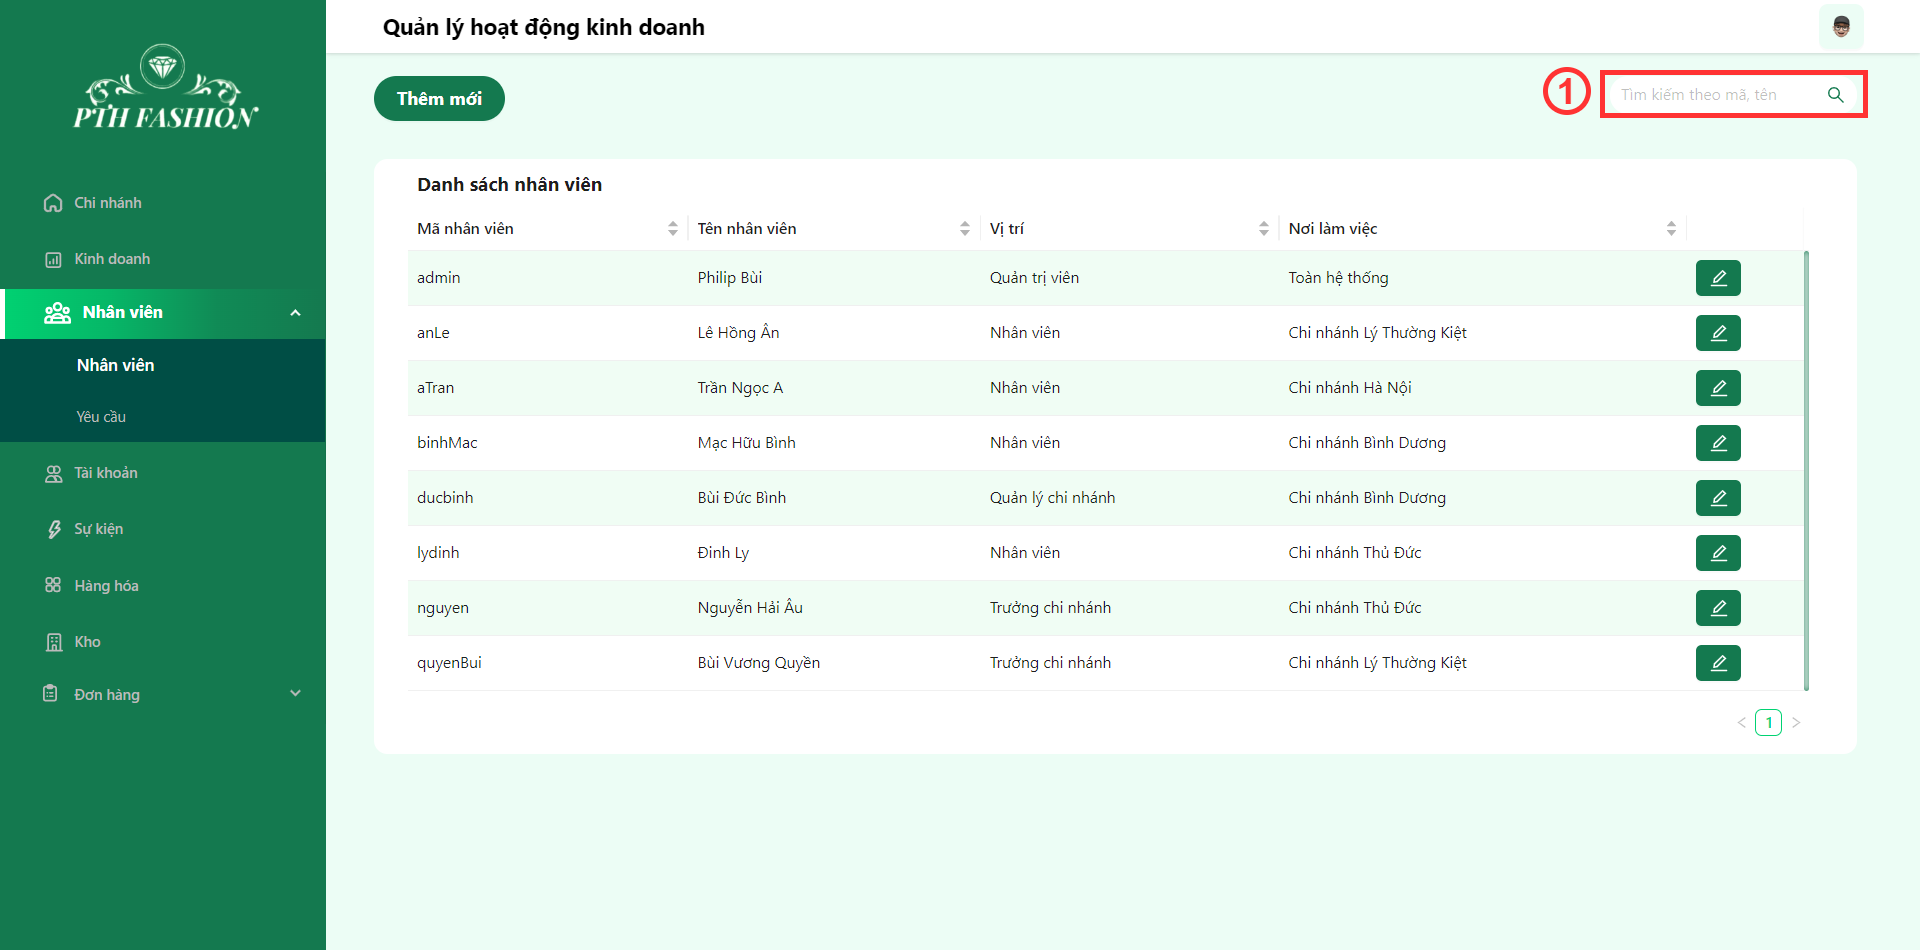
\includegraphics[width=12cm]{img/UI/admin_implement/staff.png}
    \newline
    \caption{Giao diện quản lý nhân viên}
\end{figure}
\textbf{Mô tả:}
\begin{quote}
    \begin{enumerate}
        \item Nhập để tìm kiếm nhân viên theo mã, tên
    \end{enumerate}
    Hiển thị danh sách tất cả nhân viên trong hệ thống. chức năng tìm kiếm tương tự cho các tính năng quản lý khác.
\end{quote}

\subsubsubsection{Thêm, chỉnh sửa nhân viên}
\begin{figure}[!htp]
    \centering
    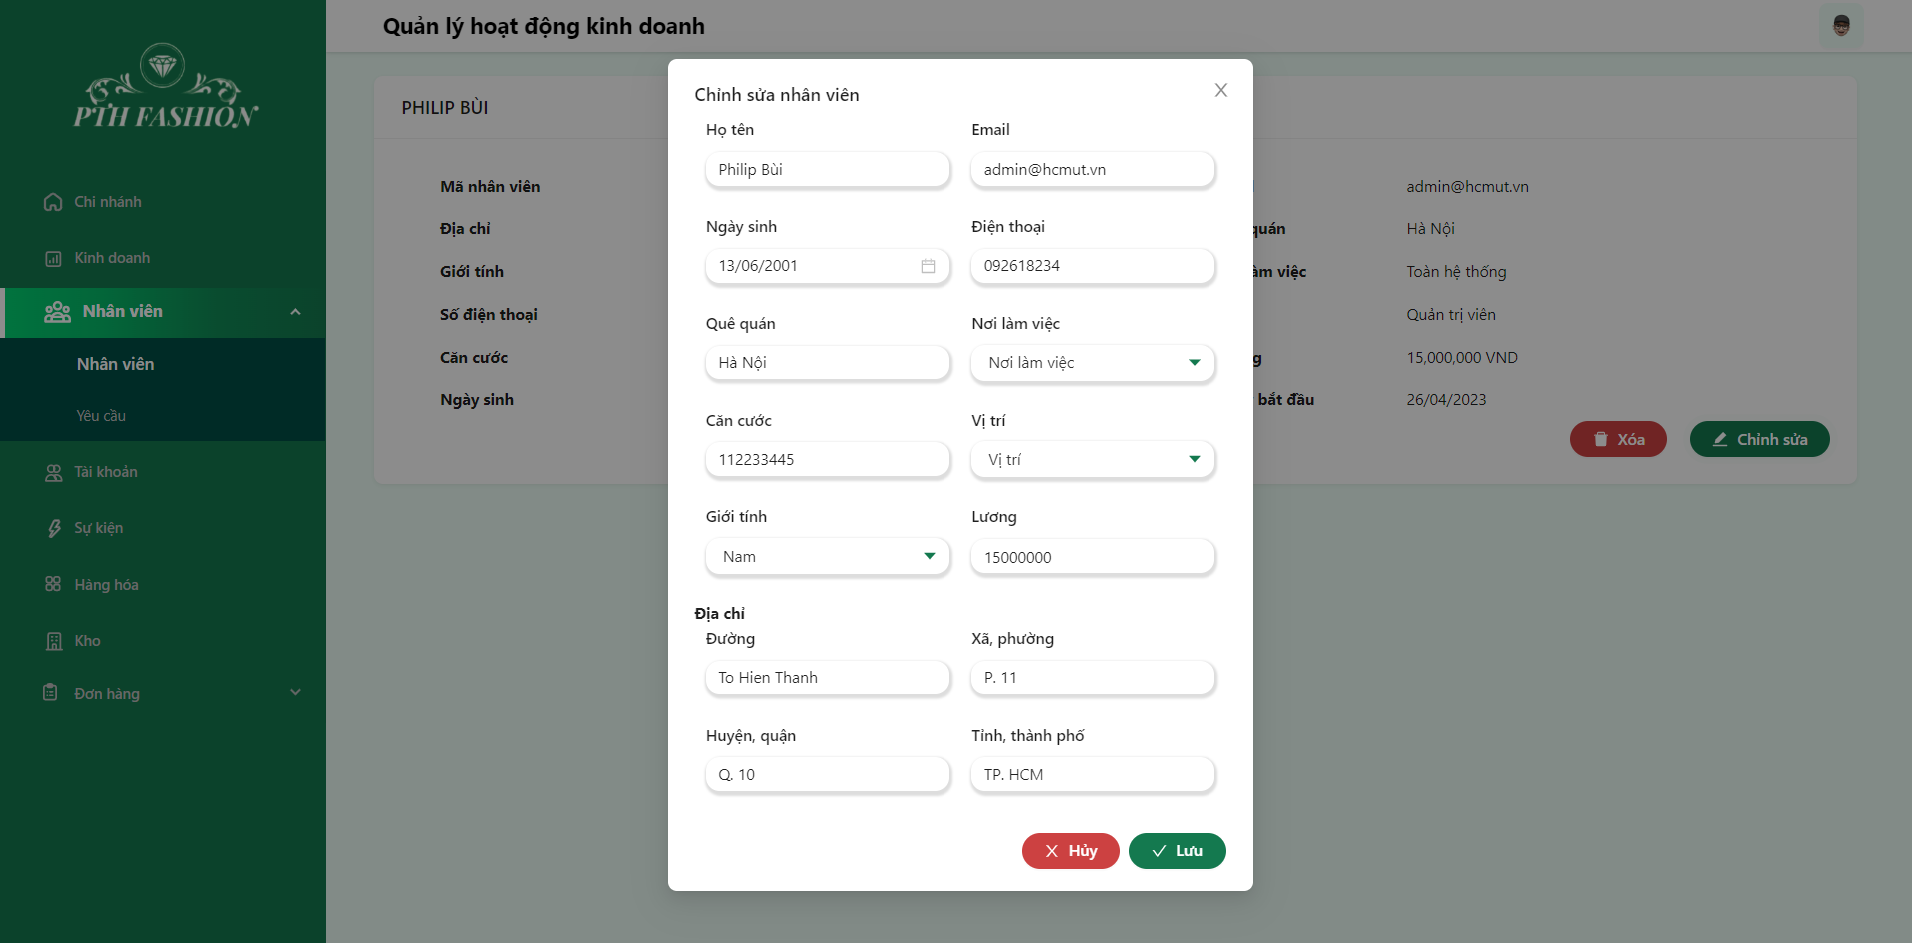
\includegraphics[width=12cm]{img/UI/admin_implement/staffEdit.png}
    \newline
    \caption{Form thêm, chỉnh sửa nhân viên}
\end{figure}


\subsubsubsection{Thông tin chi tiết nhân viên}
\begin{figure}[!htp]
    \centering
    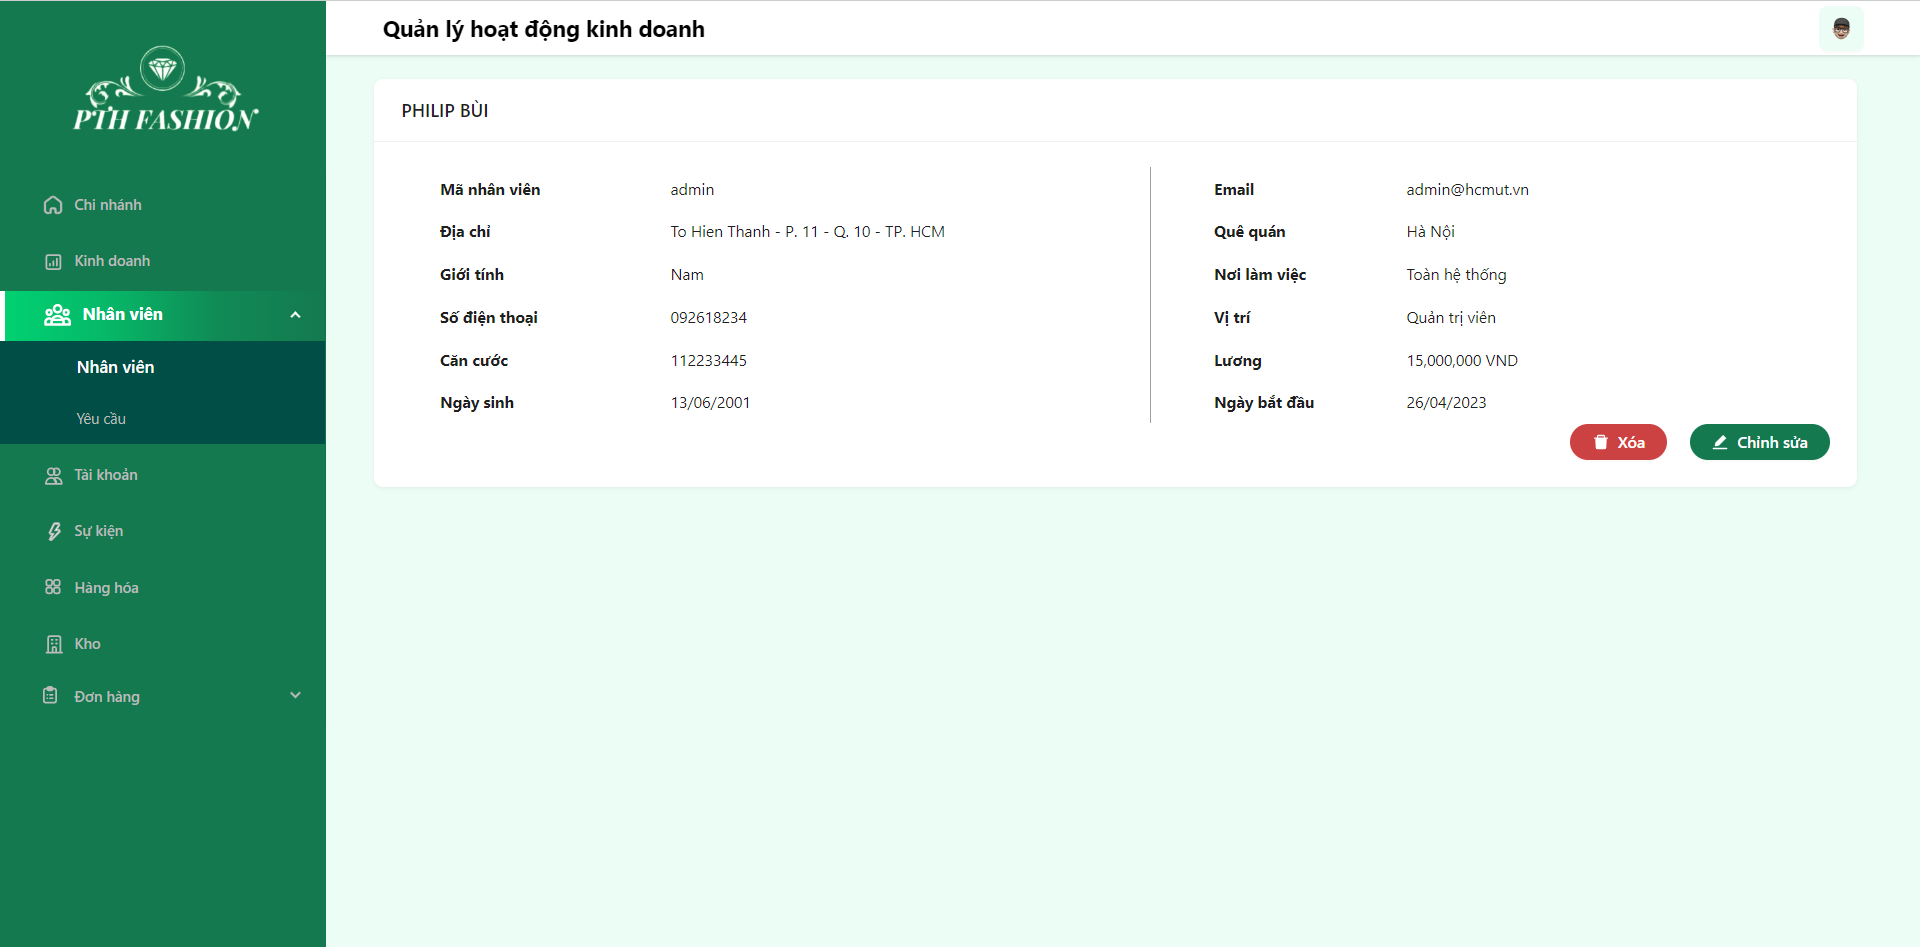
\includegraphics[width=12cm]{img/UI/admin_implement/staffDetail.png}
    \newline
    \caption{Giao diện thông tin chi tiết nhân viên}
\end{figure}
% \newpage

\subsubsubsection{Quản lý yêu cầu nhân viên}
\begin{figure}[!htp]
    \centering
    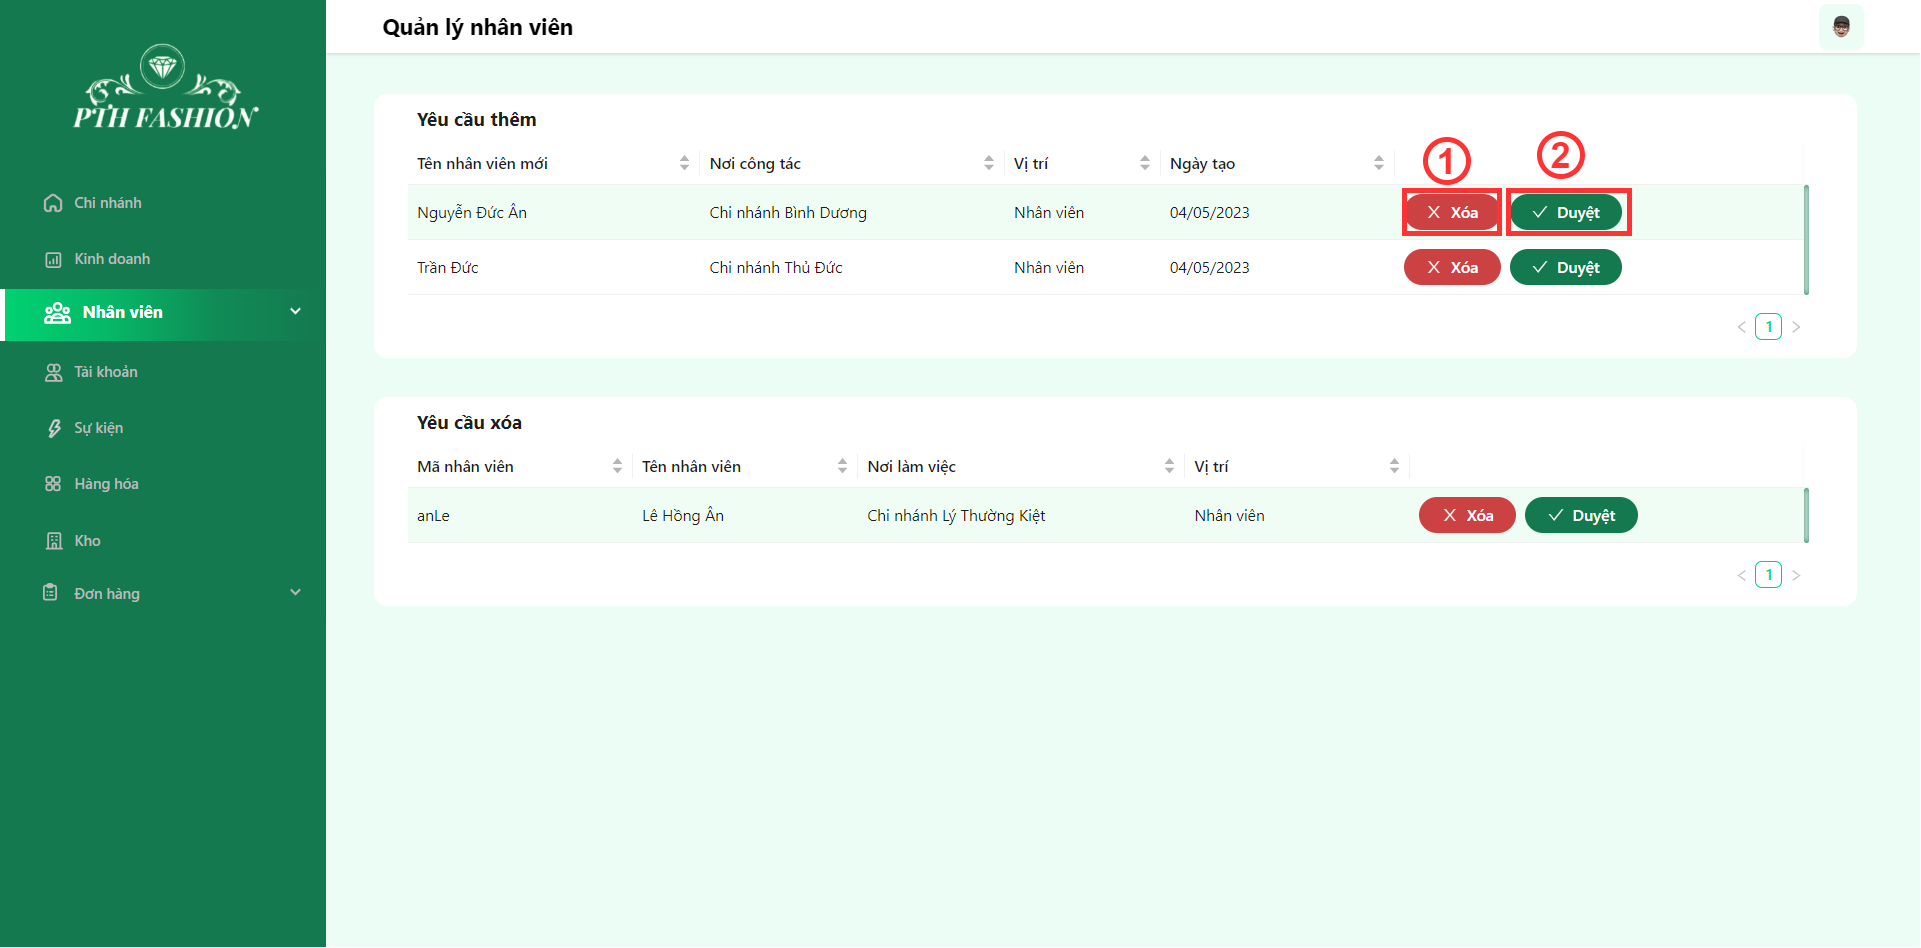
\includegraphics[width=12cm]{img/UI/admin_implement/staffRequest.png}
    \newline
    \caption{Giao diện quản lý yêu cầu nhân viên}
\end{figure}
\textbf{Mô tả:}
\begin{quote}
    \begin{enumerate}
        \item Chọn để xóa yêu cầu
        \item Chọn để duyệt yêu cầu
    \end{enumerate}
\end{quote}

\subsubsubsection{Thông tin chi tiết của yêu cầu nhân viên}
\begin{figure}[!htp]
    \centering
    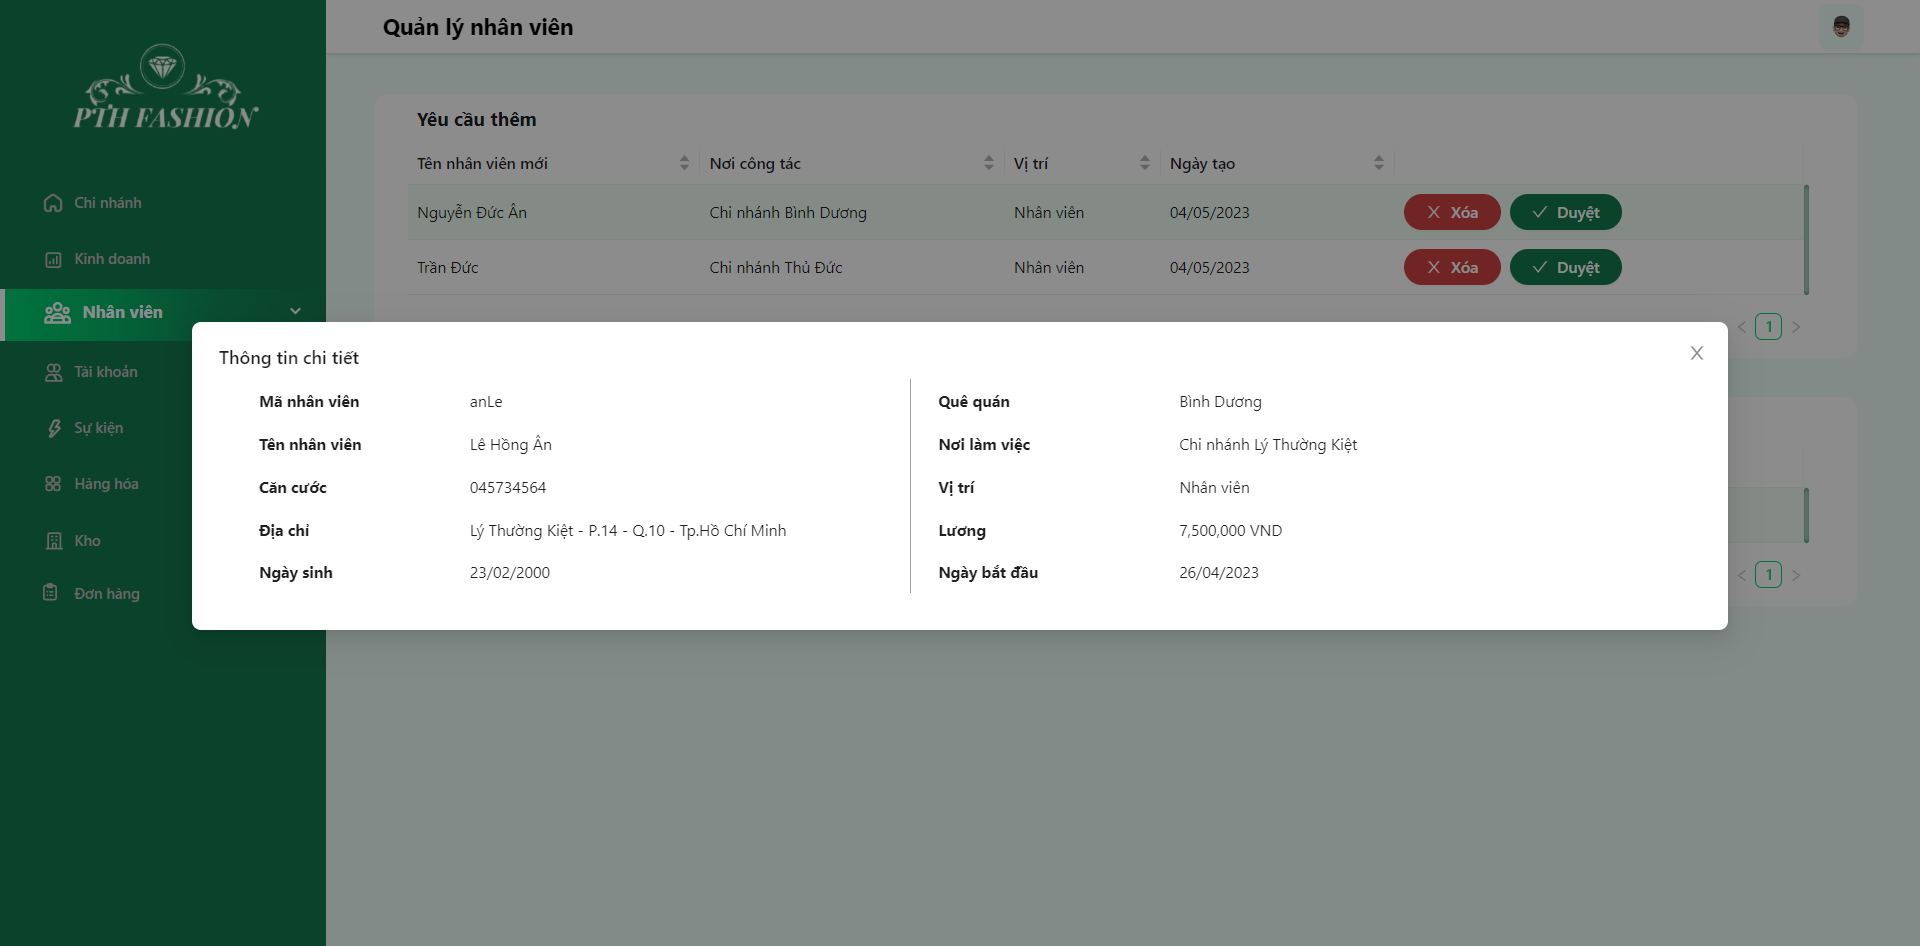
\includegraphics[width=12cm]{img/UI/admin_implement/staffRequestDetail.png}
    \newline
    \caption{Giao diện Thông tin chi tiết của yêu cầu nhân viên}
\end{figure}

% \subsubsubsection{Yêu cầu thêm nhân viên}
% \subsubsubsection{Yêu cầu xóa nhân viên}

\newpage

\subsubsection{Quản lý tài khoản}
\begin{figure}[!htp]
    \centering
    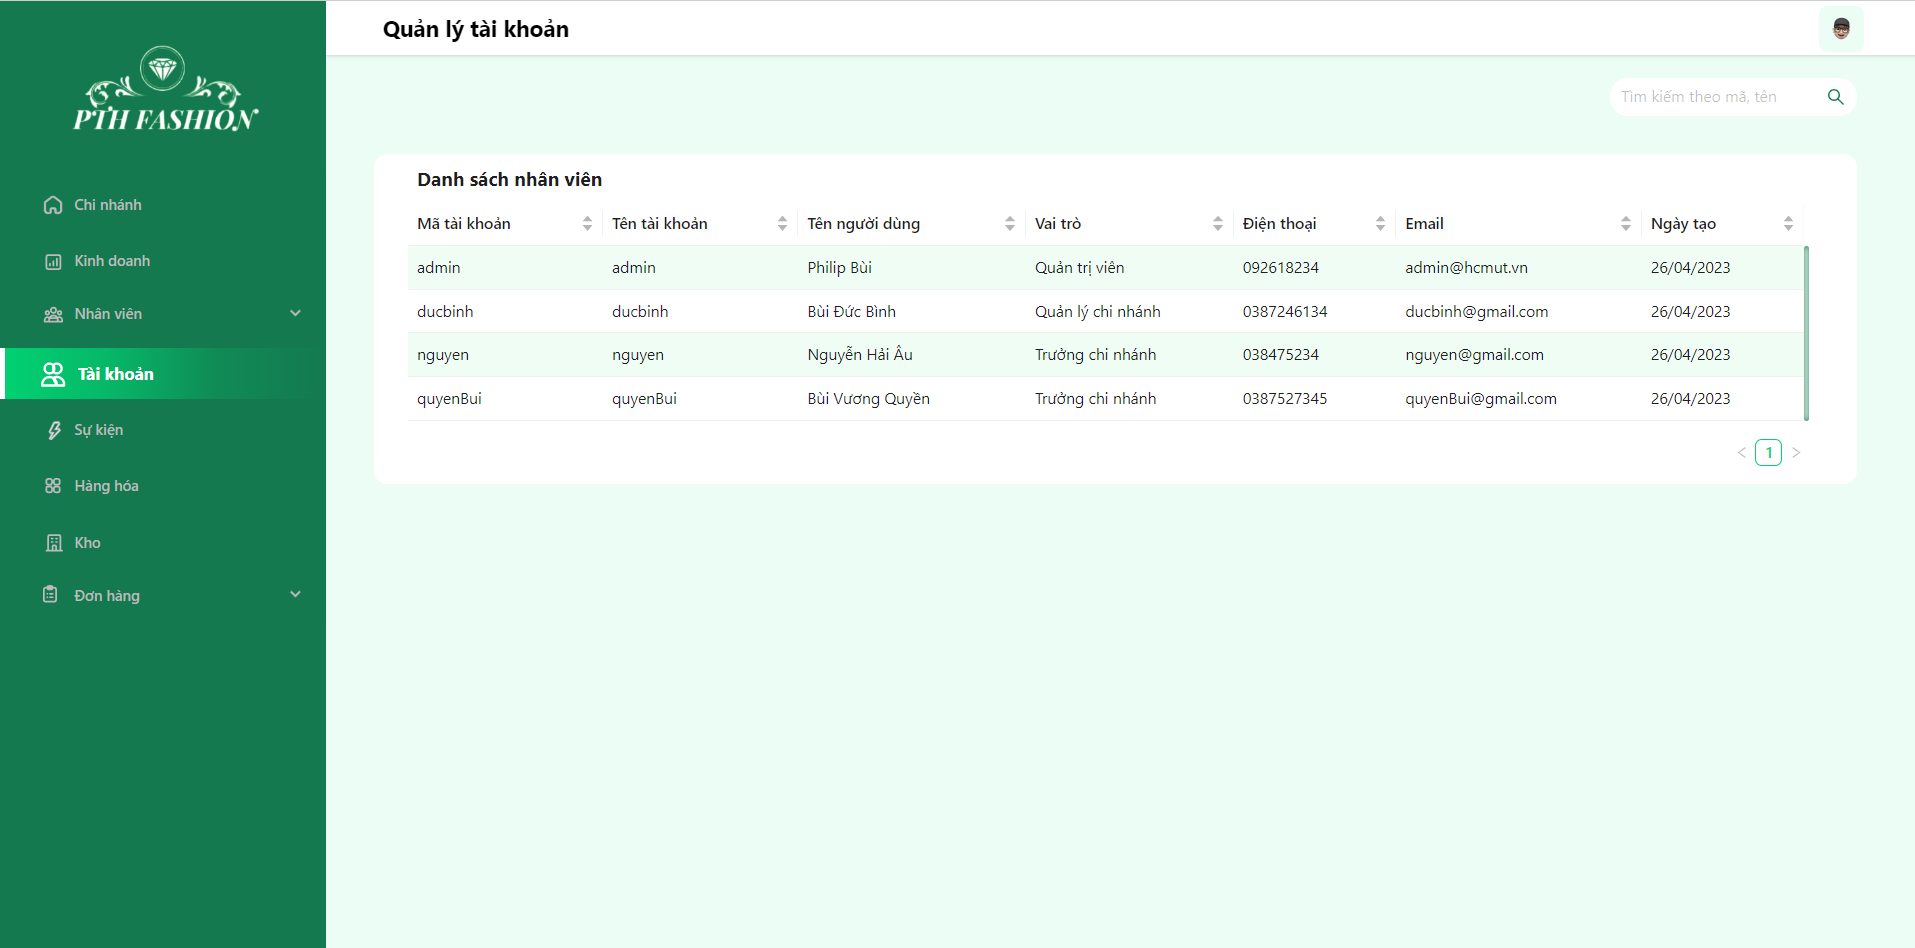
\includegraphics[width=12cm]{img/UI/admin_implement/account.png}
    \newline
    \caption{Giao diện quản lý tài khoản}
\end{figure}


\subsubsection{Quản lý kho}
\begin{figure}[!htp]
    \centering
    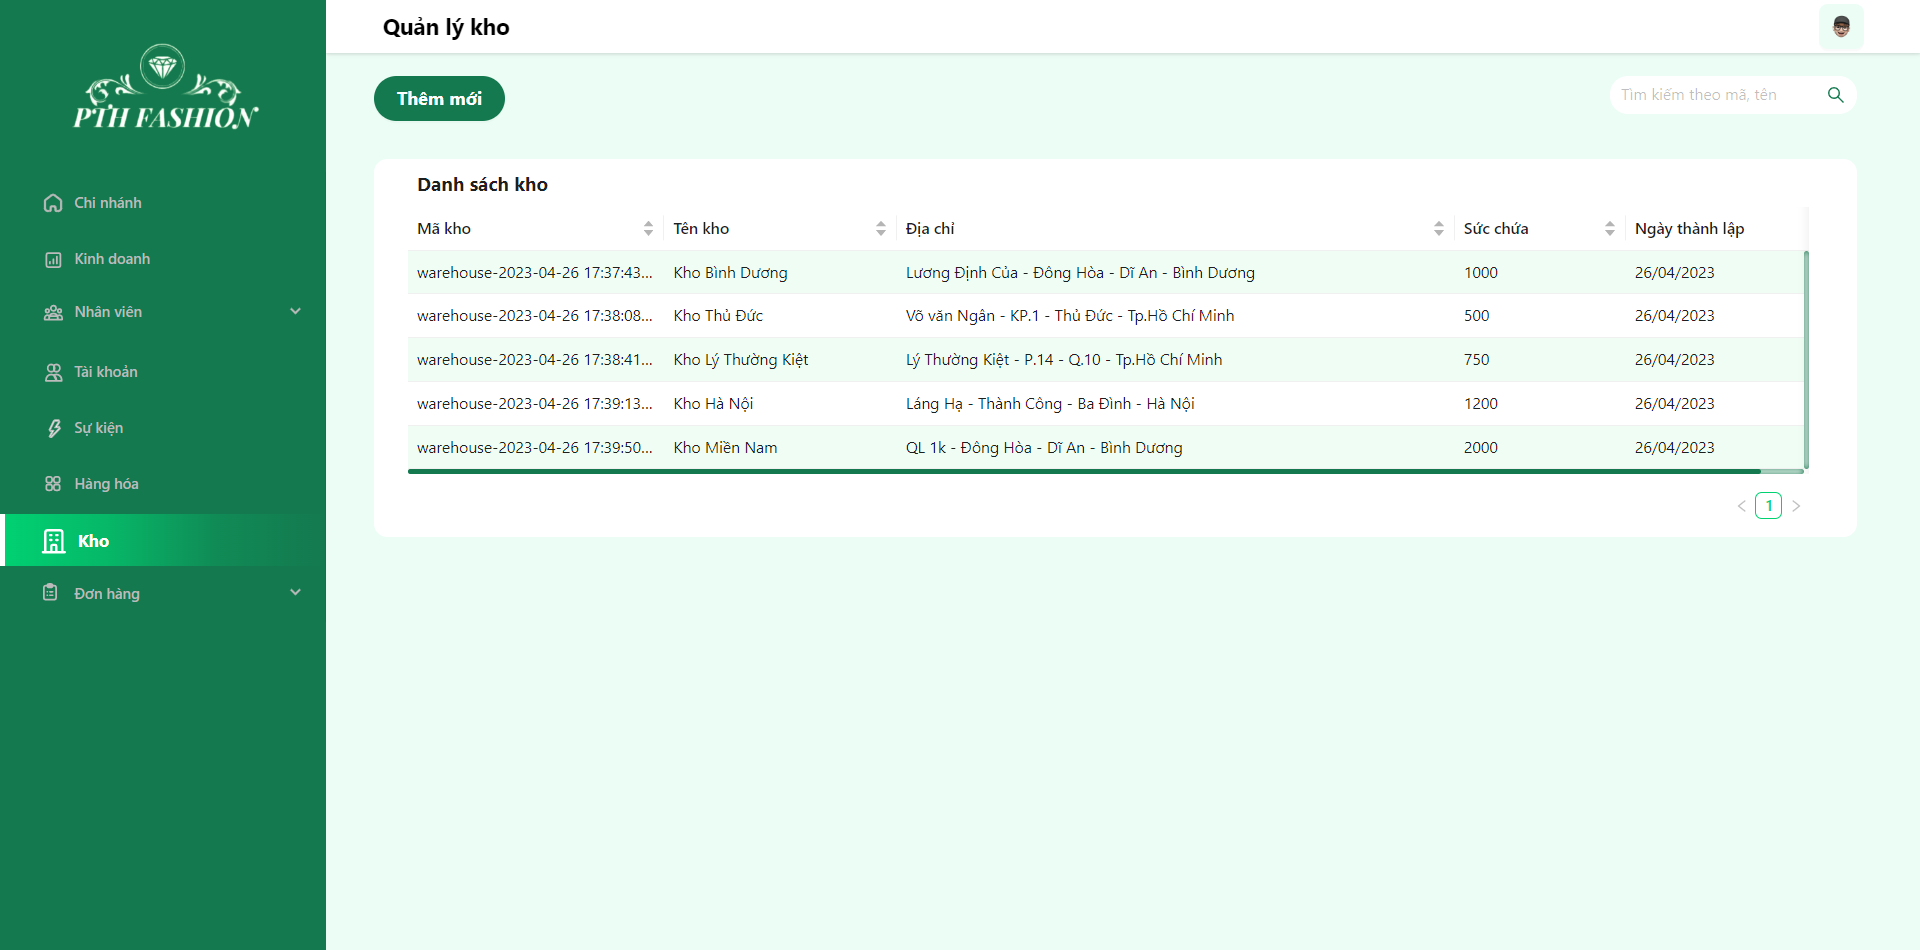
\includegraphics[width=12cm]{img/UI/admin_implement/warehouse.png}
    \newline
    \caption{Giao diện quản lý kho}
\end{figure}


\subsubsubsection{Thêm, chỉnh sửa thông tin kho}
\begin{figure}[!htp]
    \centering
    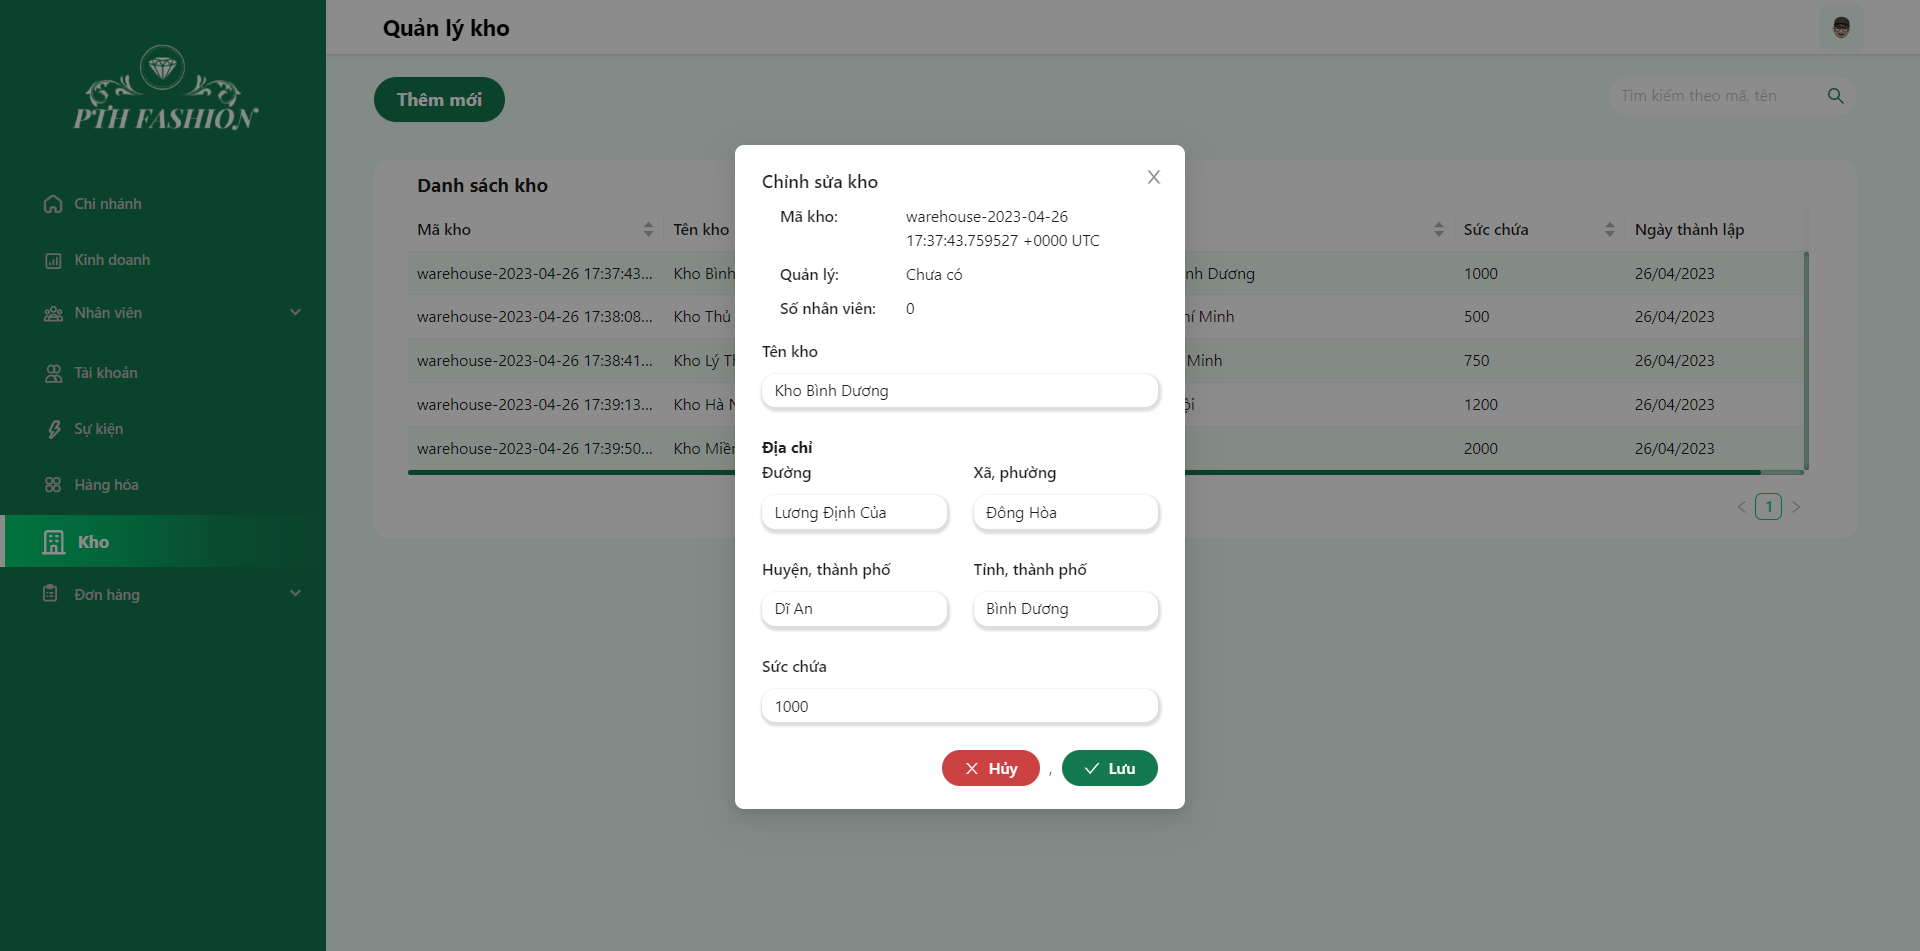
\includegraphics[width=12cm]{img/UI/admin_implement/warehouseEdit.png}
    \newline
    \caption{Giao diện thêm, chỉnh sửa thông tin kho}
\end{figure}


\newpage


\subsubsection{Quản lý sự kiện}
\begin{figure}[!htp]
    \centering
    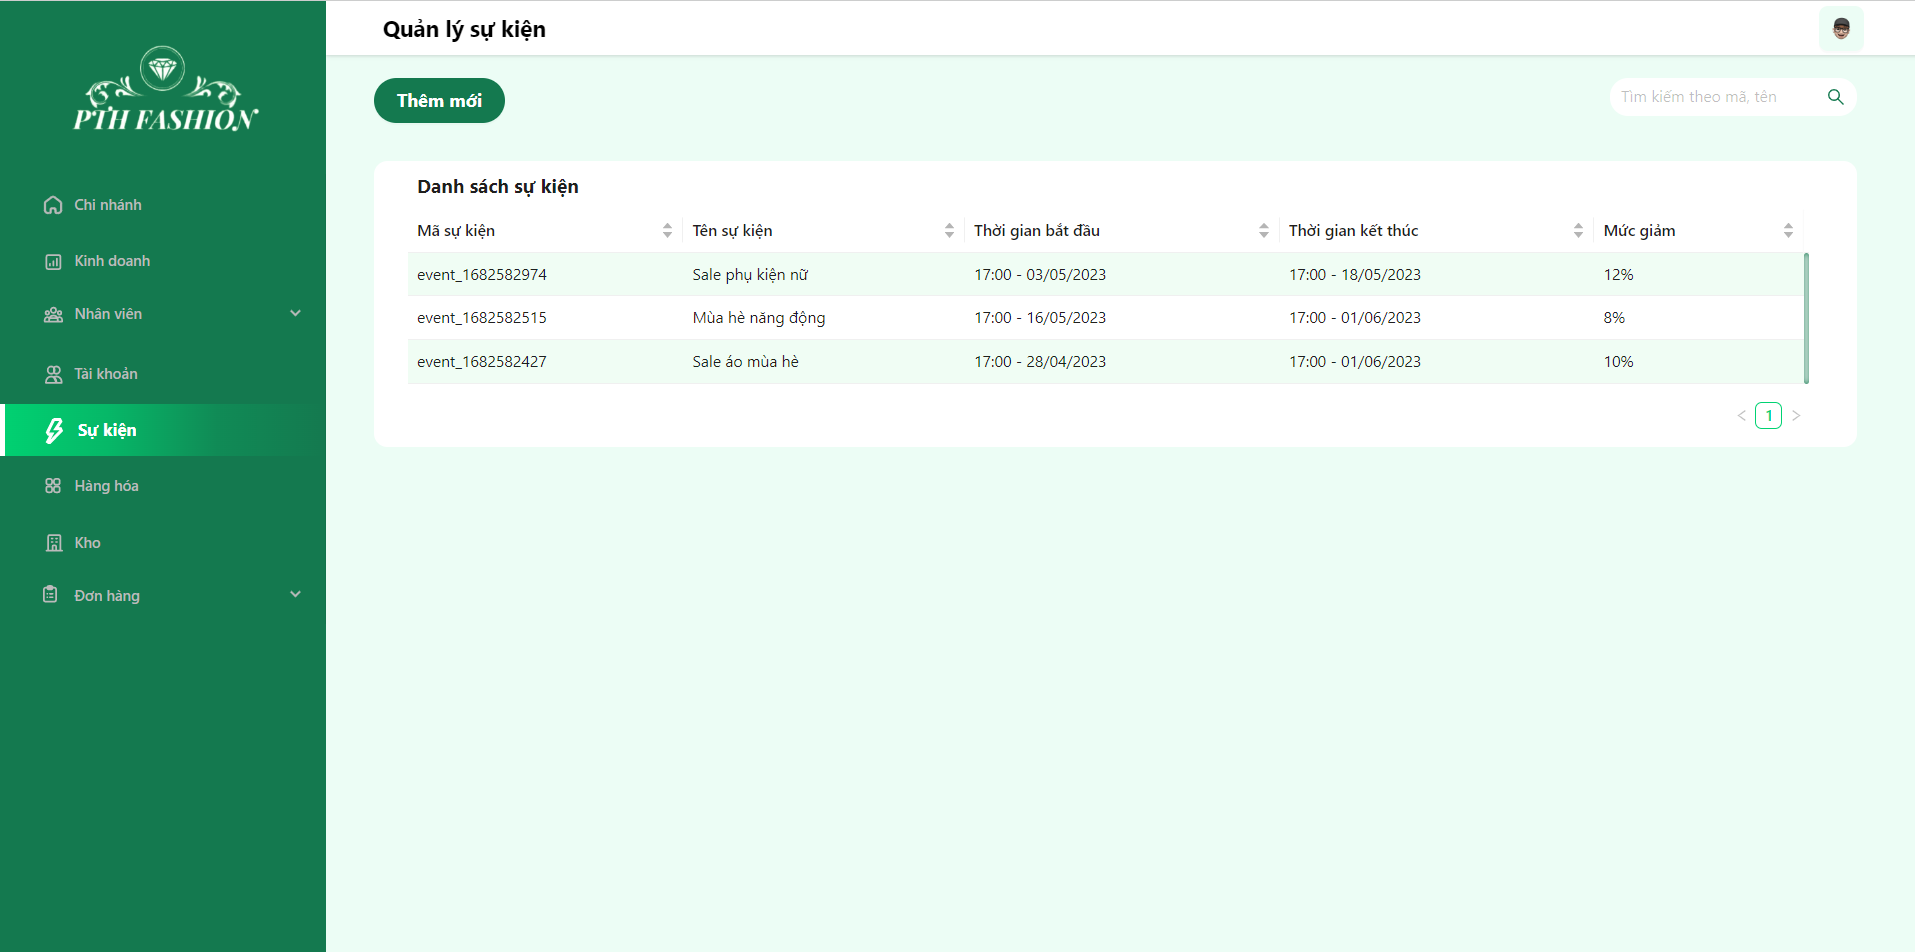
\includegraphics[width=12cm]{img/UI/admin_implement/event.png}
    \newline
    \caption{Giao diện quản lý sự kiện}
\end{figure}


\subsubsubsection{Thêm, chỉnh sửa thông tin sự kiện}
\begin{figure}[!htp]
    \centering
    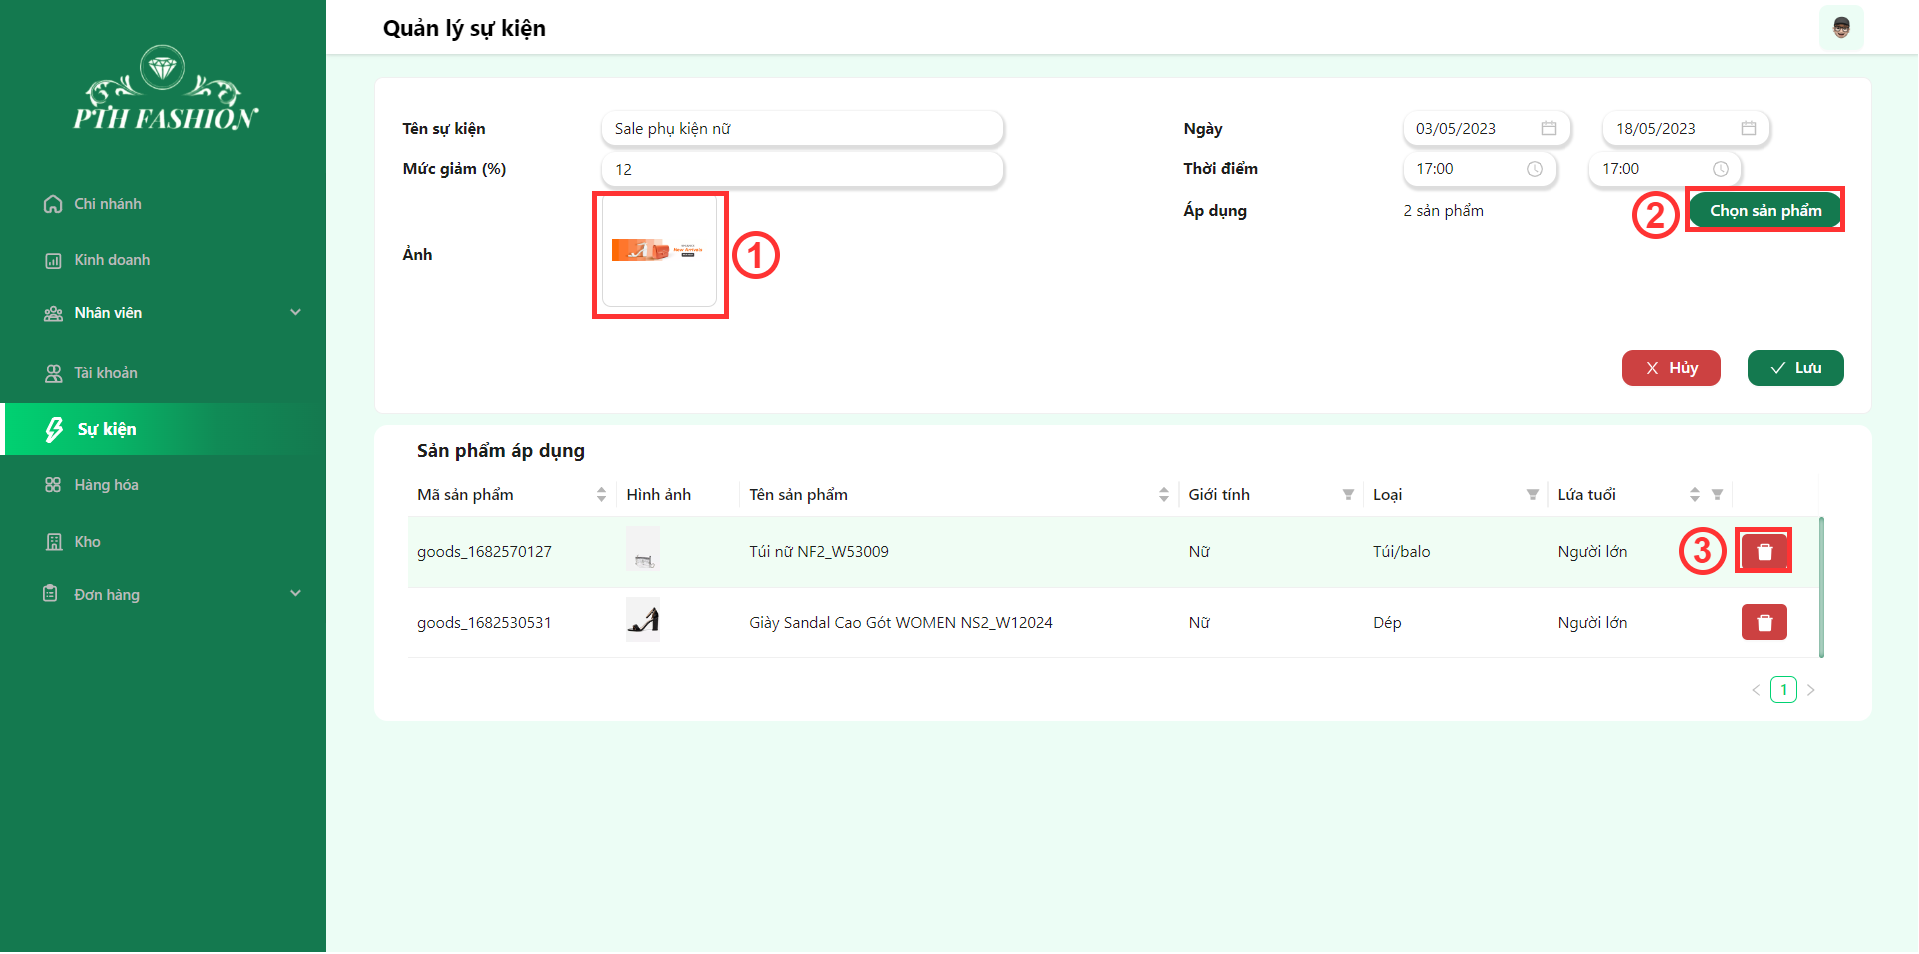
\includegraphics[width=12cm]{img/UI/admin_implement/eventEdit.png}
    \newline
    \caption{Giao diện thêm, chỉnh sửa thông tin sự kiện}
\end{figure}
\textbf{Mô tả:}
\begin{quote}
    \begin{enumerate}
        \item Chọn để tải ảnh lên cho sự kiện
        \item Chọn để chọn danh sách hàng cho sự kiện
        \item Chọn xóa hàng khỏi sự kiện
    \end{enumerate}
\end{quote}

% \newpage

\subsubsubsection{Chọn hàng cho sự kiện}
\begin{figure}[!htp]
    \centering
    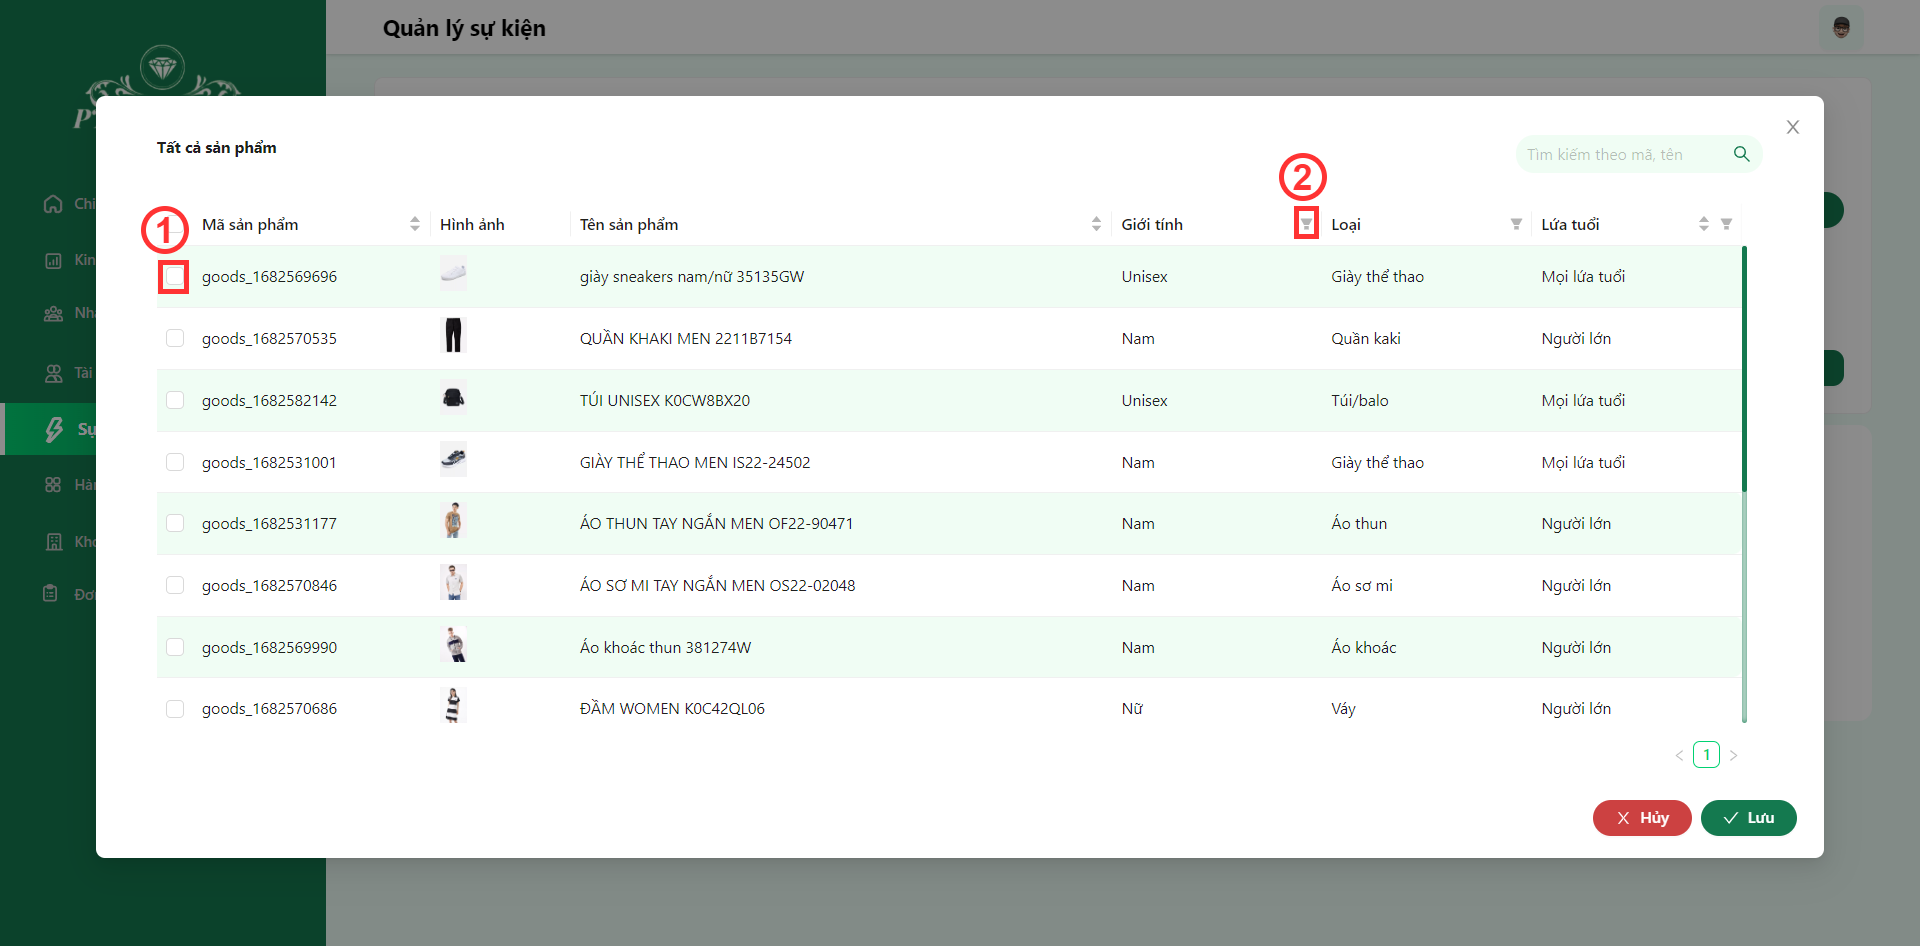
\includegraphics[width=12cm]{img/UI/admin_implement/eventAllGoods.png}
    \newline
    \caption{Giao diện chọn hàng cho sự kiện}
\end{figure}
\textbf{Mô tả:}
\begin{quote}
    \begin{enumerate}
        \item Chọn để thêm hàng cho sự kiện
        \item Chọn để lọc hàng theo loại hàng, tương tự các tính năng lọc khác
    \end{enumerate}
\end{quote}

\newpage
\subsubsection{Quản lý hàng hóa}
\begin{figure}[!htp]
    \centering
    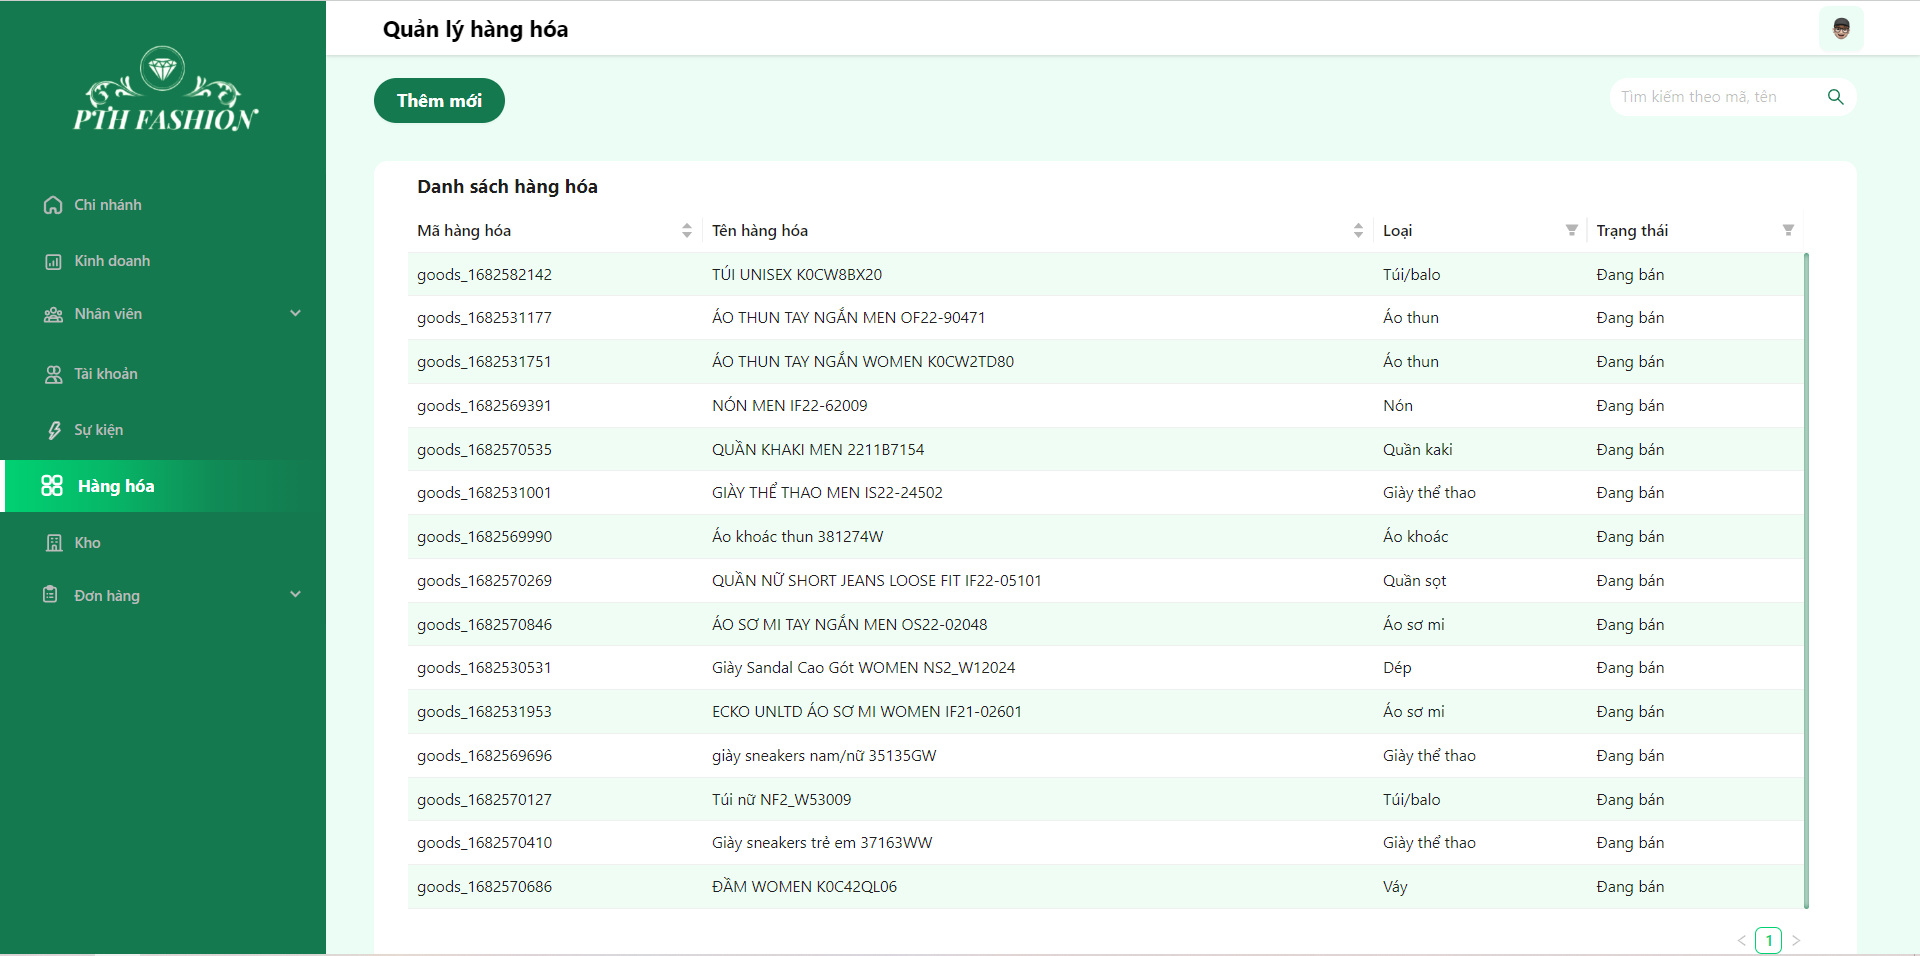
\includegraphics[width=12cm]{img/UI/admin_implement/goods.png}
    \newline
    \caption{Giao diện quản lý hàng hóa}
\end{figure}


\subsubsubsection{Thêm, chỉnh sửa thông tin hàng}
\begin{figure}[!htp]
    \centering
    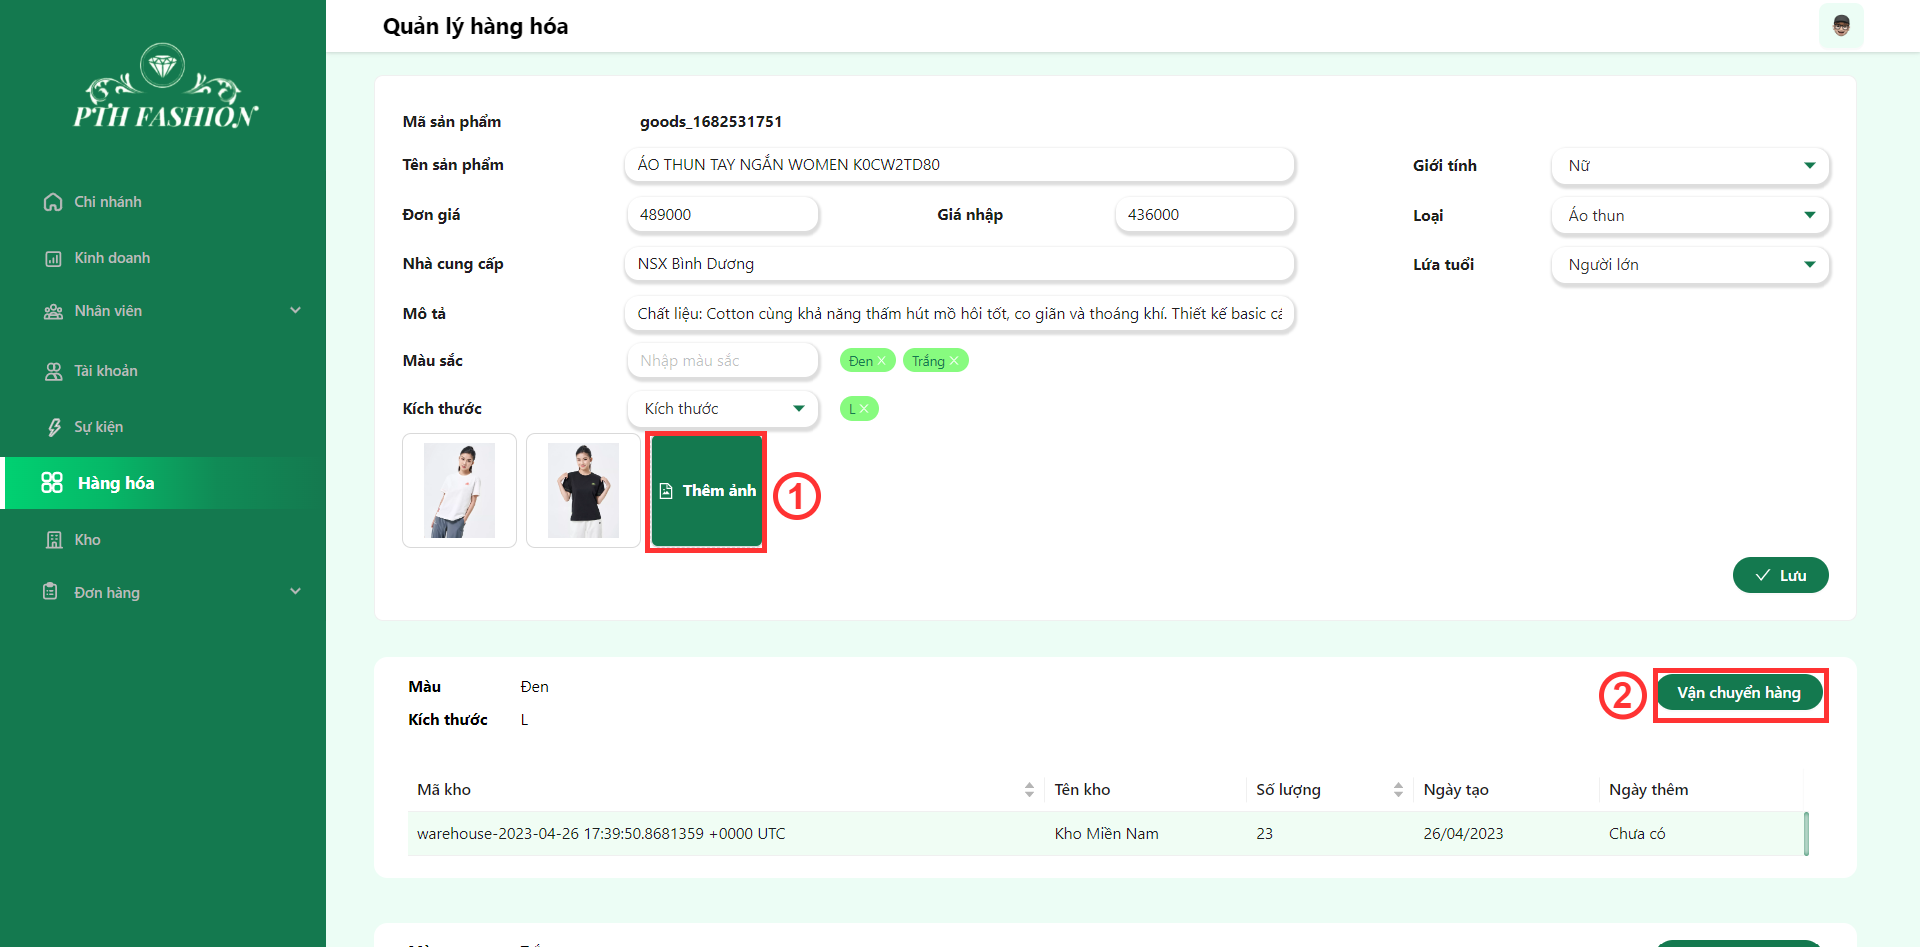
\includegraphics[width=12cm]{img/UI/admin_implement/goodsEdit.png}
    \newline
    \caption{Giao diện thêm mới, chỉnh sửa thông tin hàng}
\end{figure}
\textbf{Mô tả:}
\begin{quote}
    \begin{enumerate}
        \item Chọn để mở modal thêm ảnh cho hàng
        \item Chọn để mở modal vận chuyển hàng hàng
    \end{enumerate}
\end{quote}

\subsubsubsection{Thêm ảnh cho hàng hàng}
\begin{figure}[!htp]
    \centering
    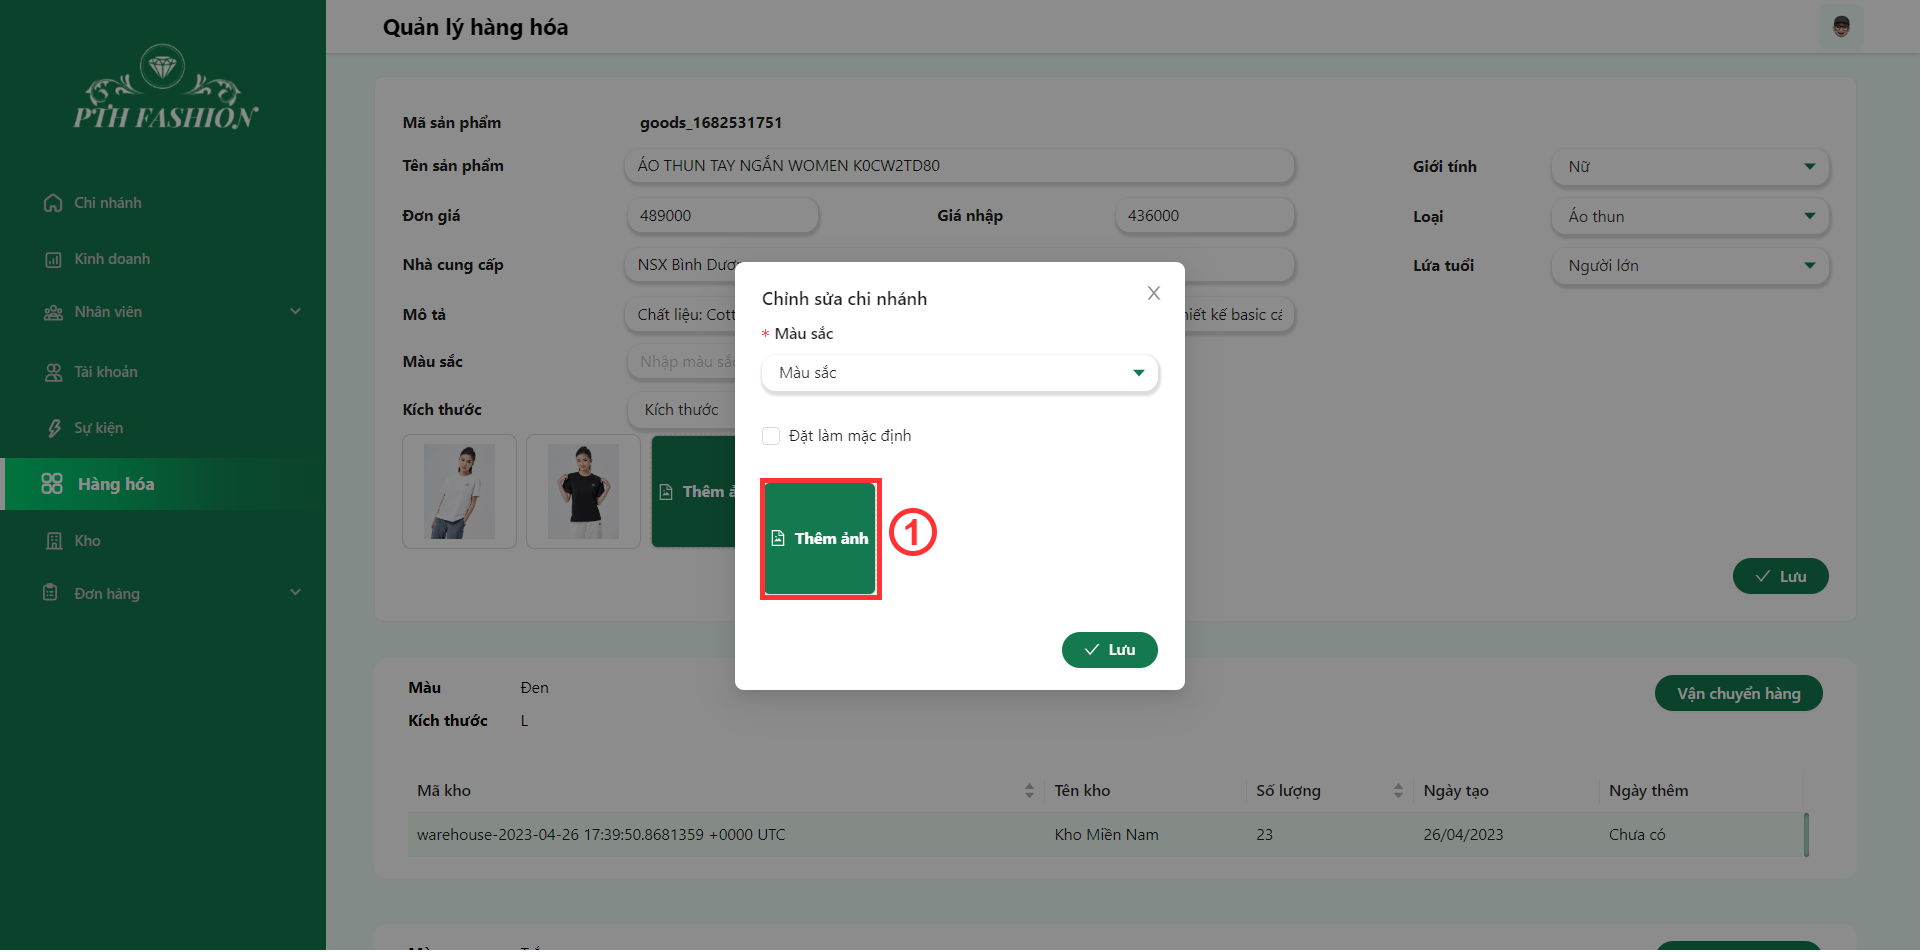
\includegraphics[width=12cm]{img/UI/admin_implement/goodsImage.png}
    \newline
    \caption{Giao diện thêm ảnh cho hàng}
\end{figure}
\textbf{Mô tả:}
\begin{quote}
    \begin{enumerate}
        \item Chọn để tải ảnh lên
    \end{enumerate}
\end{quote}

\subsubsubsection{Vận chuyển hàng}
\begin{figure}[!htp]
    \centering
    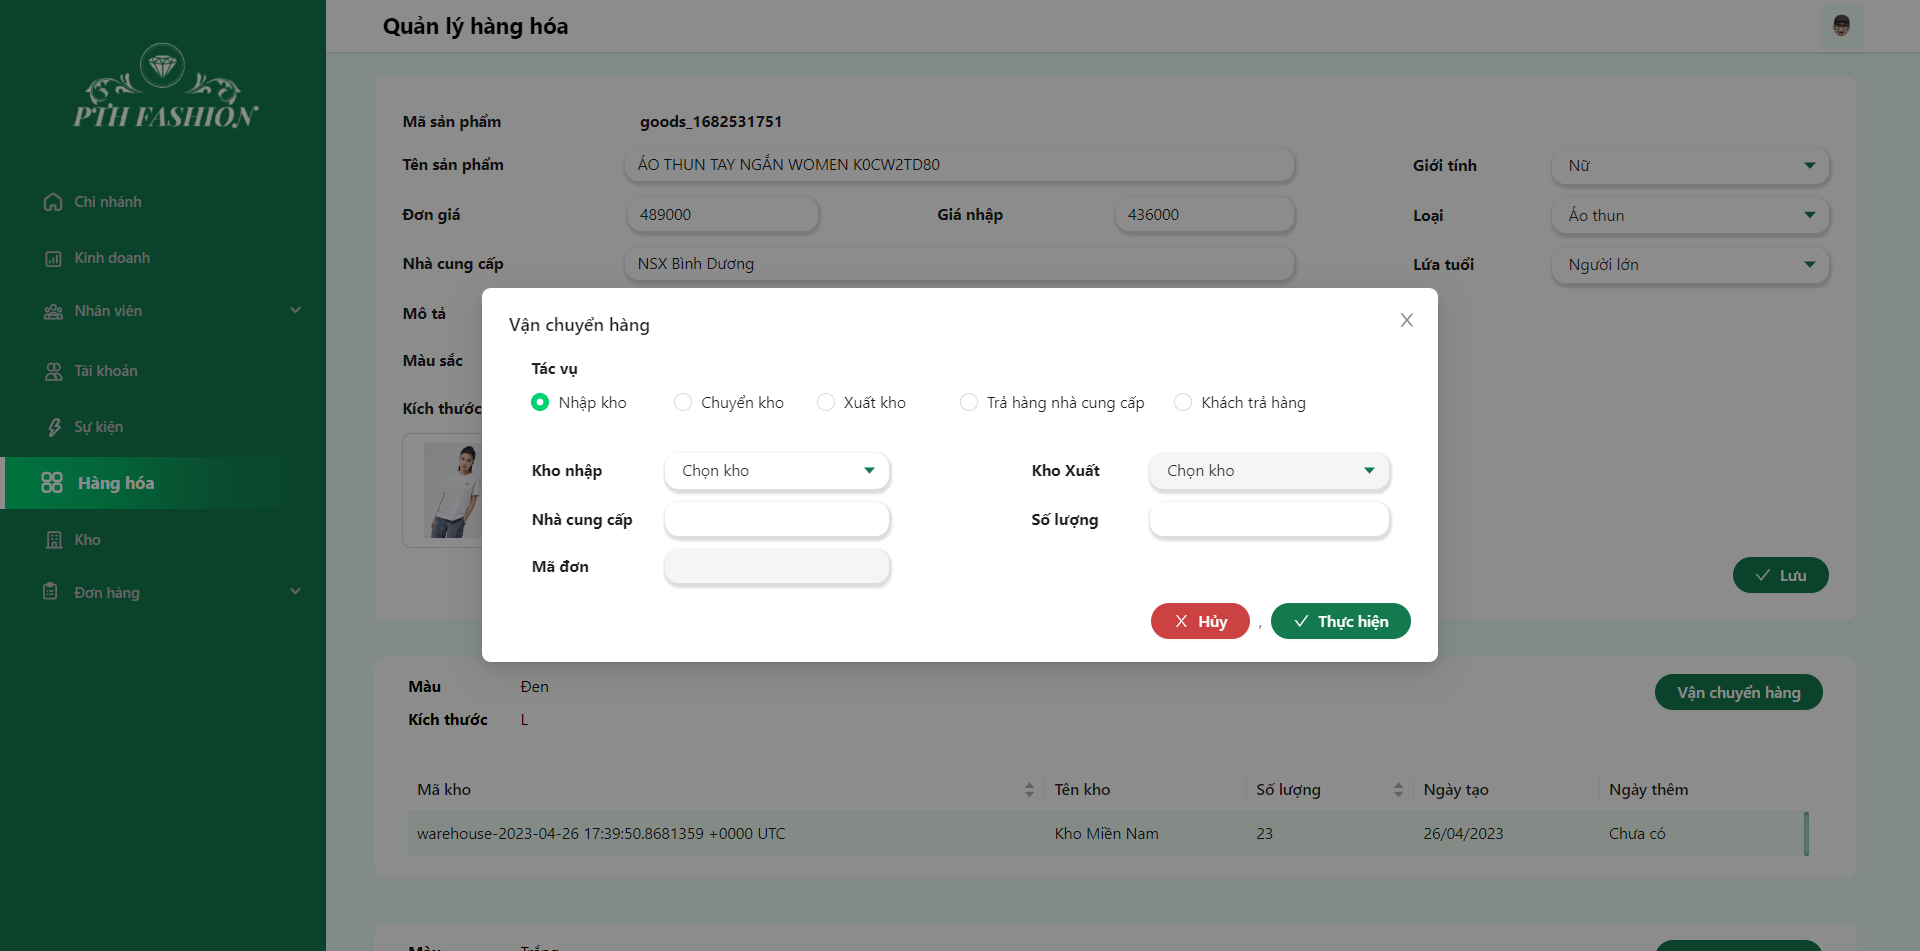
\includegraphics[width=12cm]{img/UI/admin_implement/goodsTransfer.png}
    \newline
    \caption{Giao diện vận chuyển hàng}
\end{figure}
\textbf{Mô tả:}
\begin{quote}
    Người dùng có thể thực hiện nhập kho, chuyển kho, xuất kho, nhận hàng và trả hàng
\end{quote}

\newpage

\subsubsection{Quản lý đơn hàng}
\begin{figure}[!htp]
    \centering
    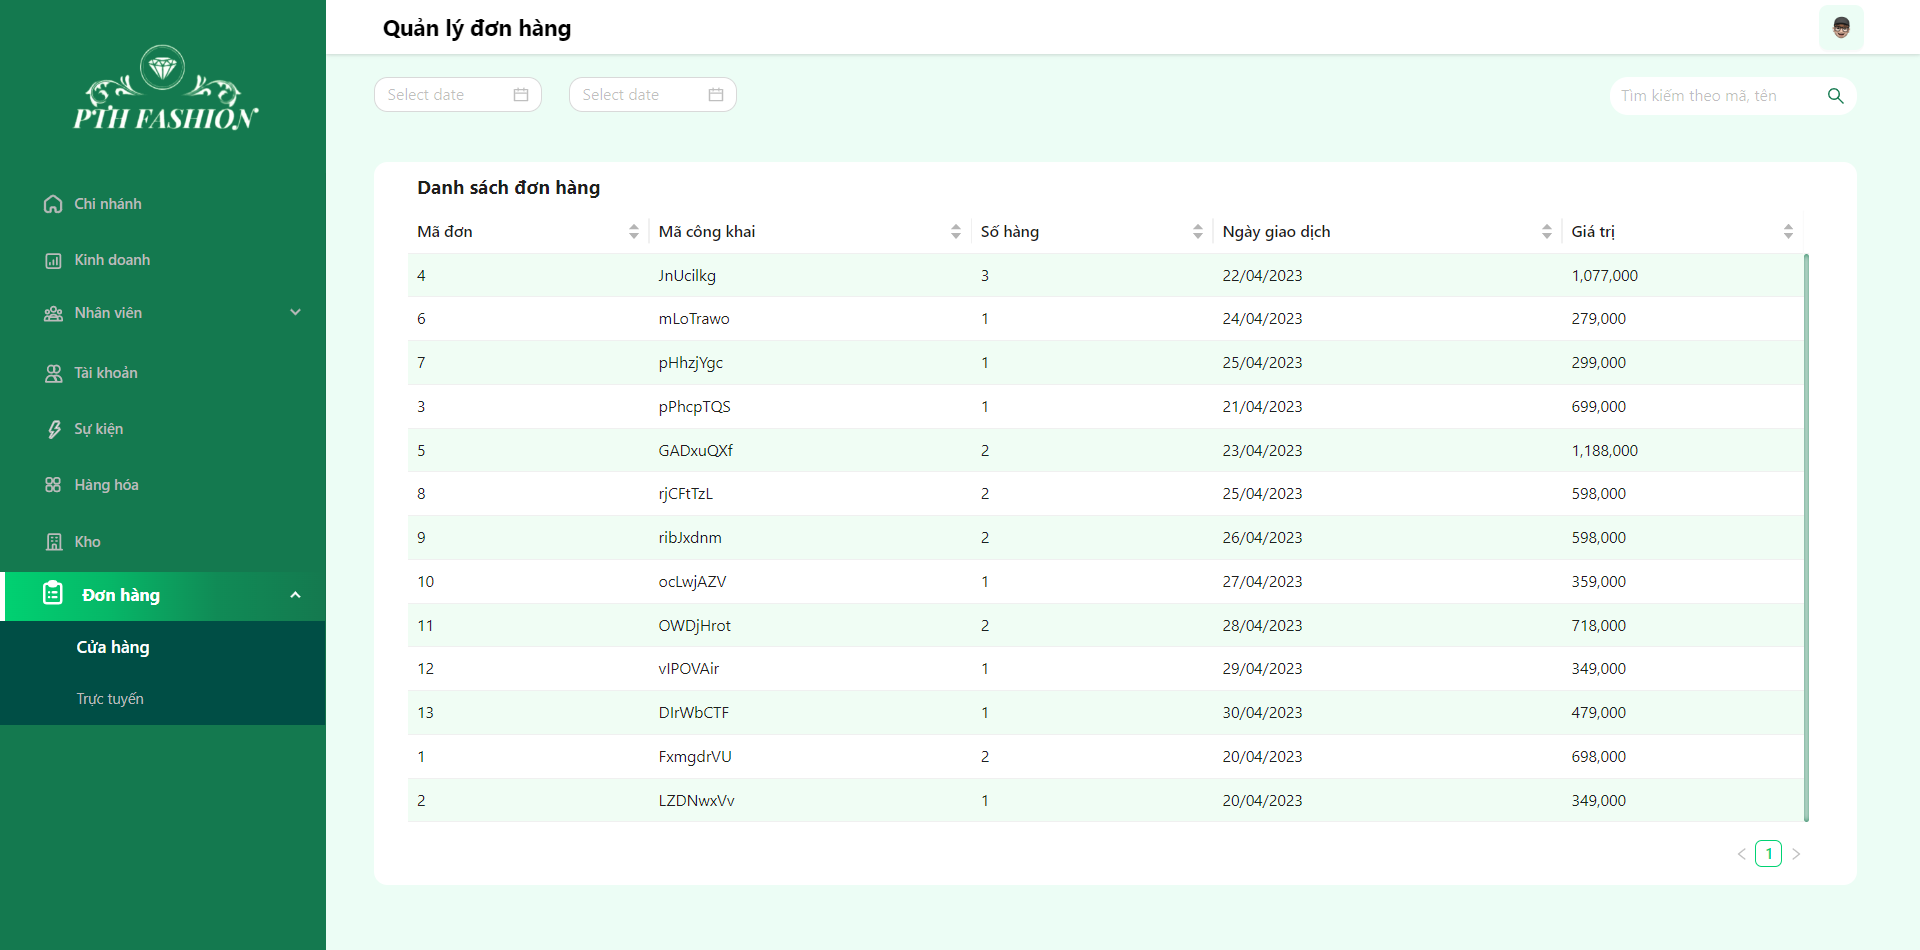
\includegraphics[width=12cm]{img/UI/admin_implement/order.png}
    \newline
    \caption{Giao diện quản lý đơn hàng}
\end{figure}

\subsubsubsection{Chi tiết đơn hàng}
\begin{figure}[!htp]
    \centering
    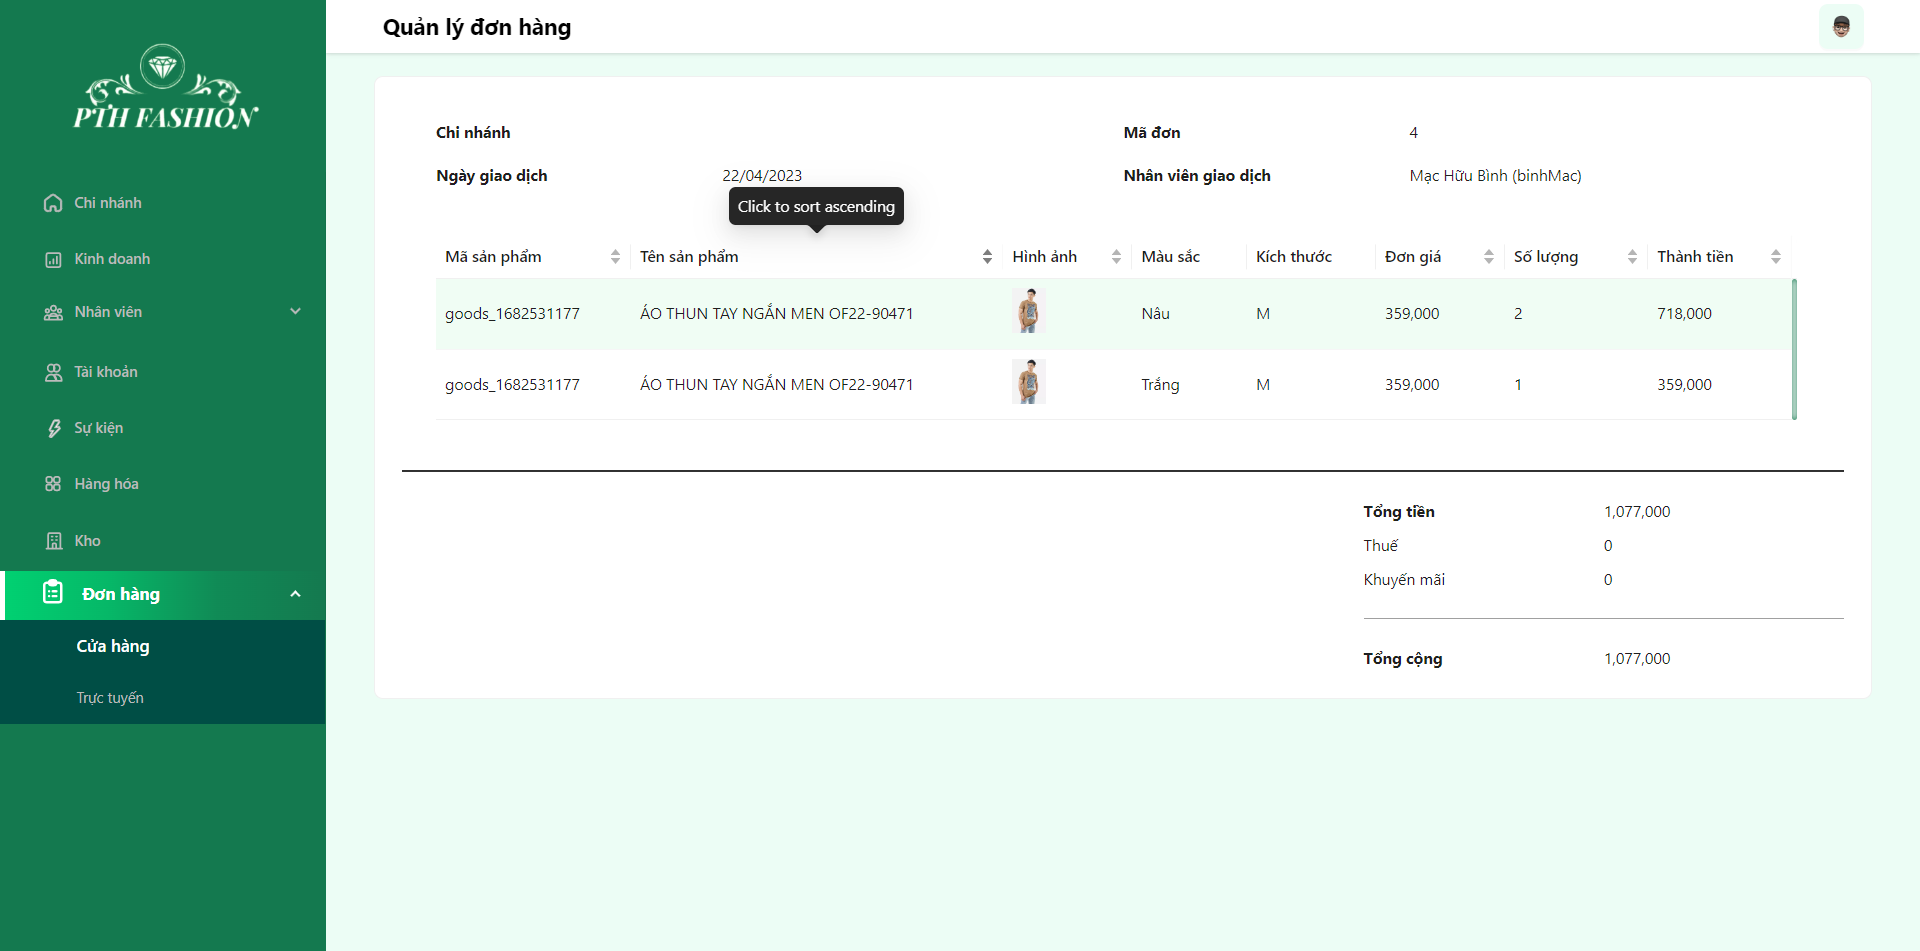
\includegraphics[width=12cm]{img/UI/admin_implement/orderDetail.png}
    \newline
    \caption{Giao diện chi tiết đơn hàng}
\end{figure}

\newpage

% \subsubsection{Quản lý đơn hàng trực tiếp}
% \begin{figure}[!htp]
%     \centering
%     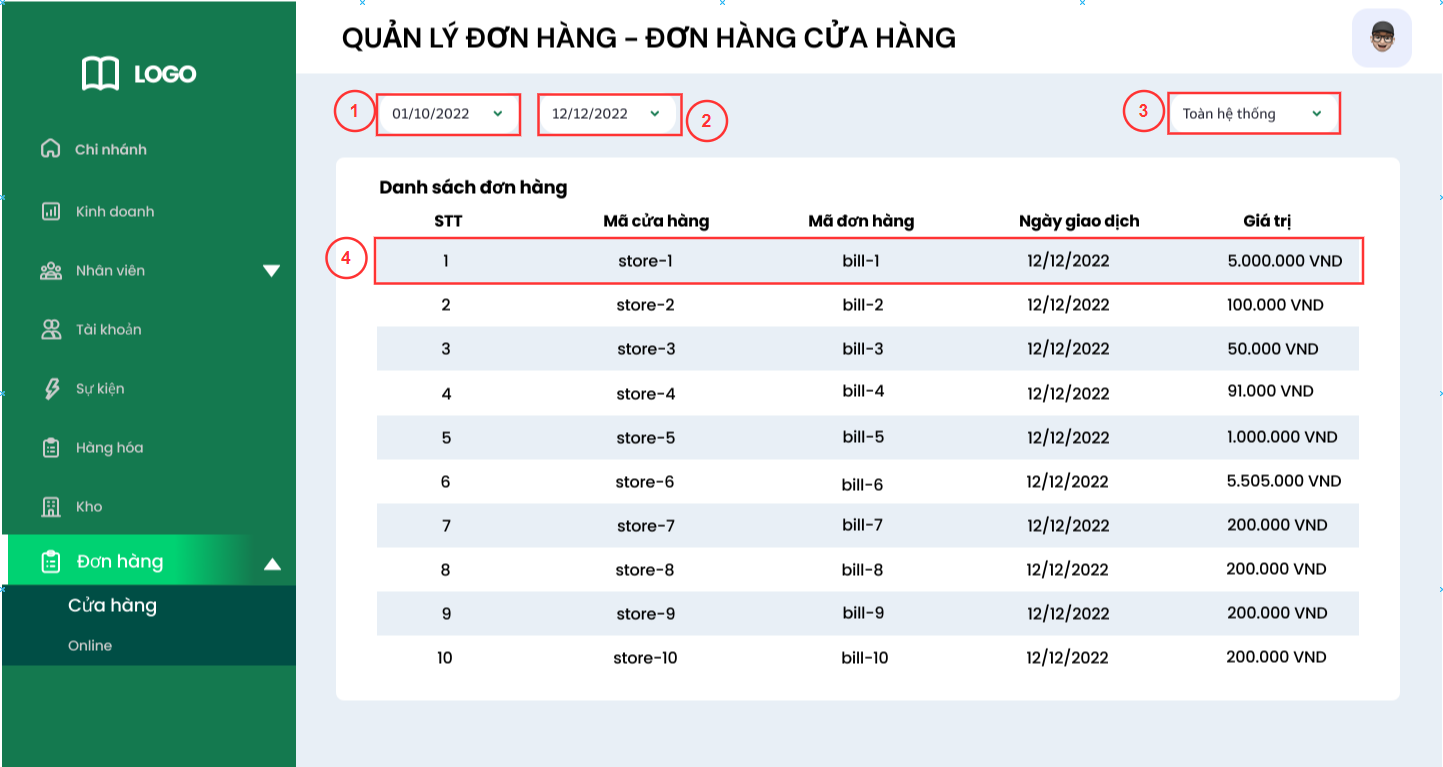
\includegraphics[width=12cm]{img/UI/admin/OfflineOrder.png}
%     \label{42}
%     \newline
%     \caption{Giao diện quản lý đơn hàng cửa hàng}
% \end{figure}
% \textbf{Mô tả:}
% \begin{quote}
%     \begin{enumerate}
%         \item Chọn thời gian bắt đầu
%         \item Chọn thời gian kết thúc
%         \item Nhập để lọc đơn theo mã đơn
%         \item Chọn để xem chi tiết đơn hàng
%     \end{enumerate}
% \end{quote}
% \subsubsubsection{Chi tiết đơn hàng cửa hàng}
% \begin{figure}[!htp]
%     \centering
%     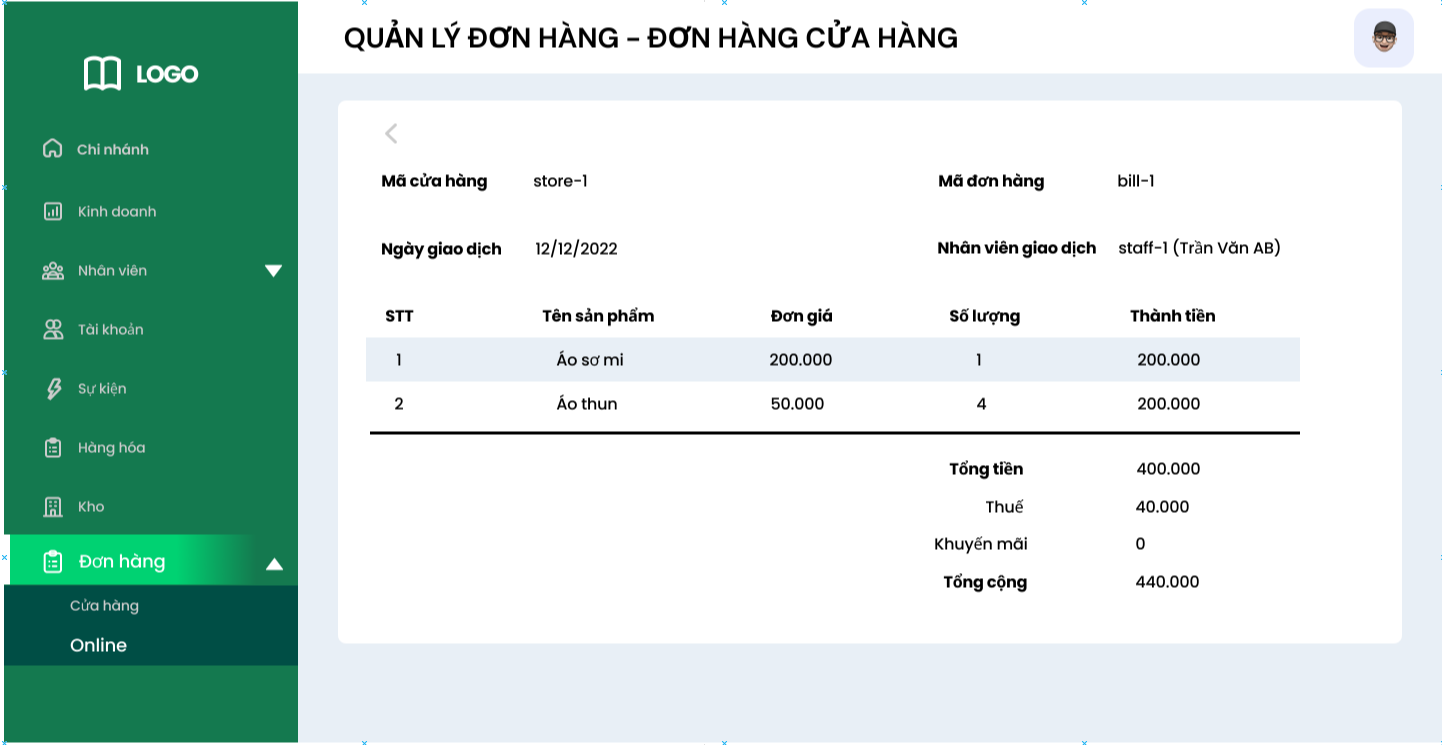
\includegraphics[width=12cm]{img/UI/admin/OfflineOrder_detai;.png}
%     \label{43}
%     \newline
%     \caption{Giao diện chi tiết đơn hàng cửa hàng}
% \end{figure}


% \subsubsection{Giao diện khác}
% Bên cạnh quản trị viên, quản lý ở cấp cao nhất thì còn các quản lý ở từng mảng và chỉ sử dụng được một vài chức năng của quản trị viên nên chỉ có sự khác nhau về phần sidebar:
% \begin{itemize}
%     \item Quản lý chi nhánh: Quản lý chi nhánh, quản lý hoạt động kinh doanh, quản lý nhân viên, quản lý đơn hàng cửa hàng
%     \item Trưởng chi nhánh: Quản lý hoạt động kinh doanh (riêng chi nhánh), quản lý nhân viên(riêng chi nhánh), quản lý đơn hàng(riêng chi nhánh).
%     \item Quản lý hàng hóa: Quản lý hàng hóa
%     \item Quản lý kho: Quản lý kho, quản lý nhân viên kho
% \end{itemize}
% \subsubsubsection{Quản lý chi nhánh}
% \begin{figure}[!htp]
%     \centering
%     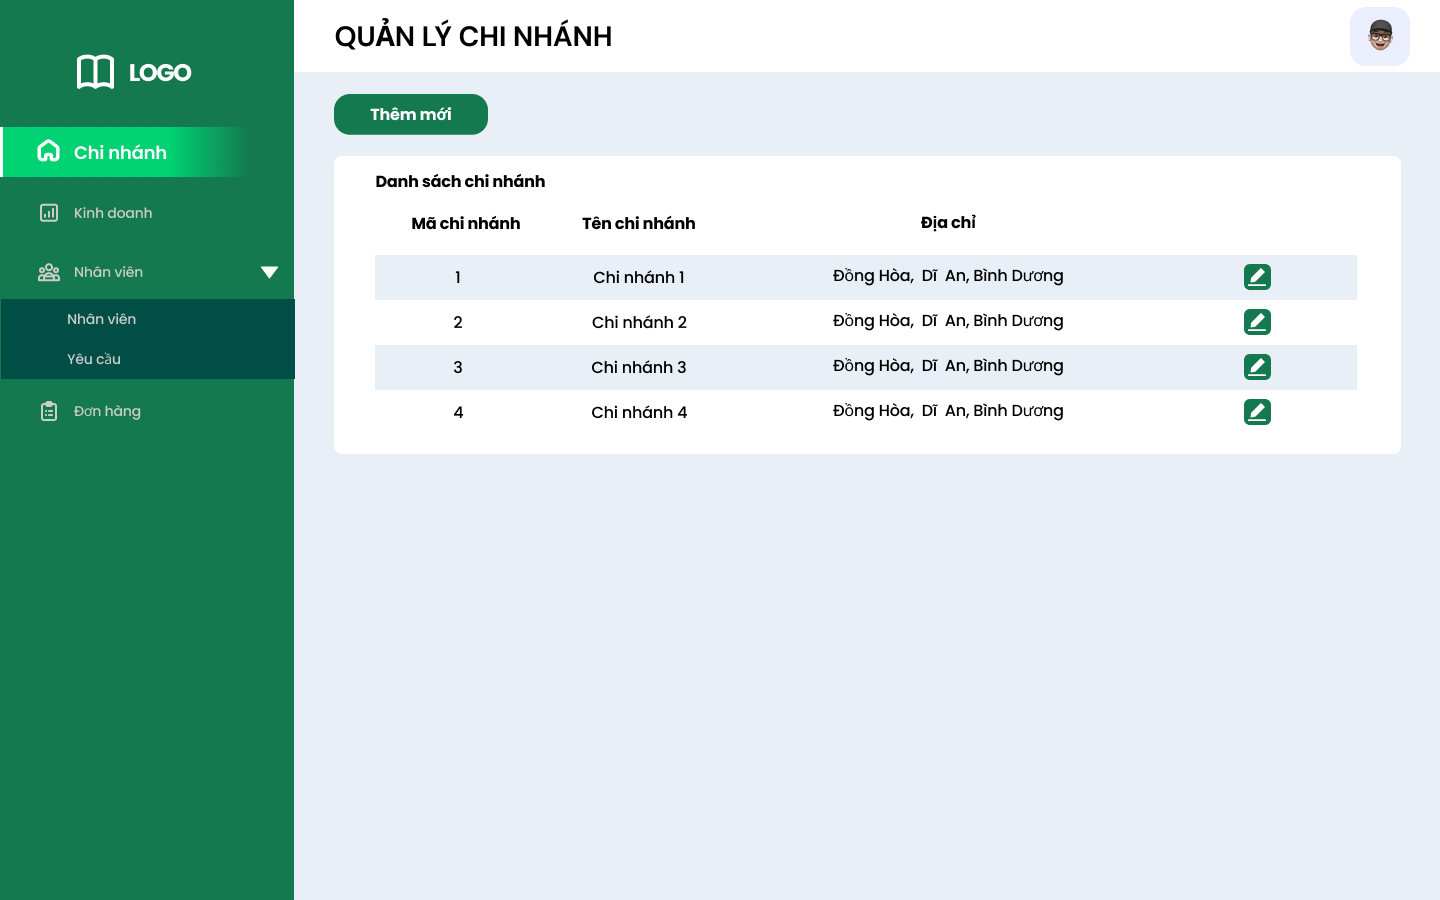
\includegraphics[width=12cm]{img/UI/admin/sub-admin. Quản lý chi nhánh.png}
%     \label{44}
%     \newline
%     \caption{Giao diện của người quản lý chi nhánh}
% \end{figure}

% \subsubsubsection{Trưởng chi nhánh}
% \begin{figure}[!htp]
%     \centering
%     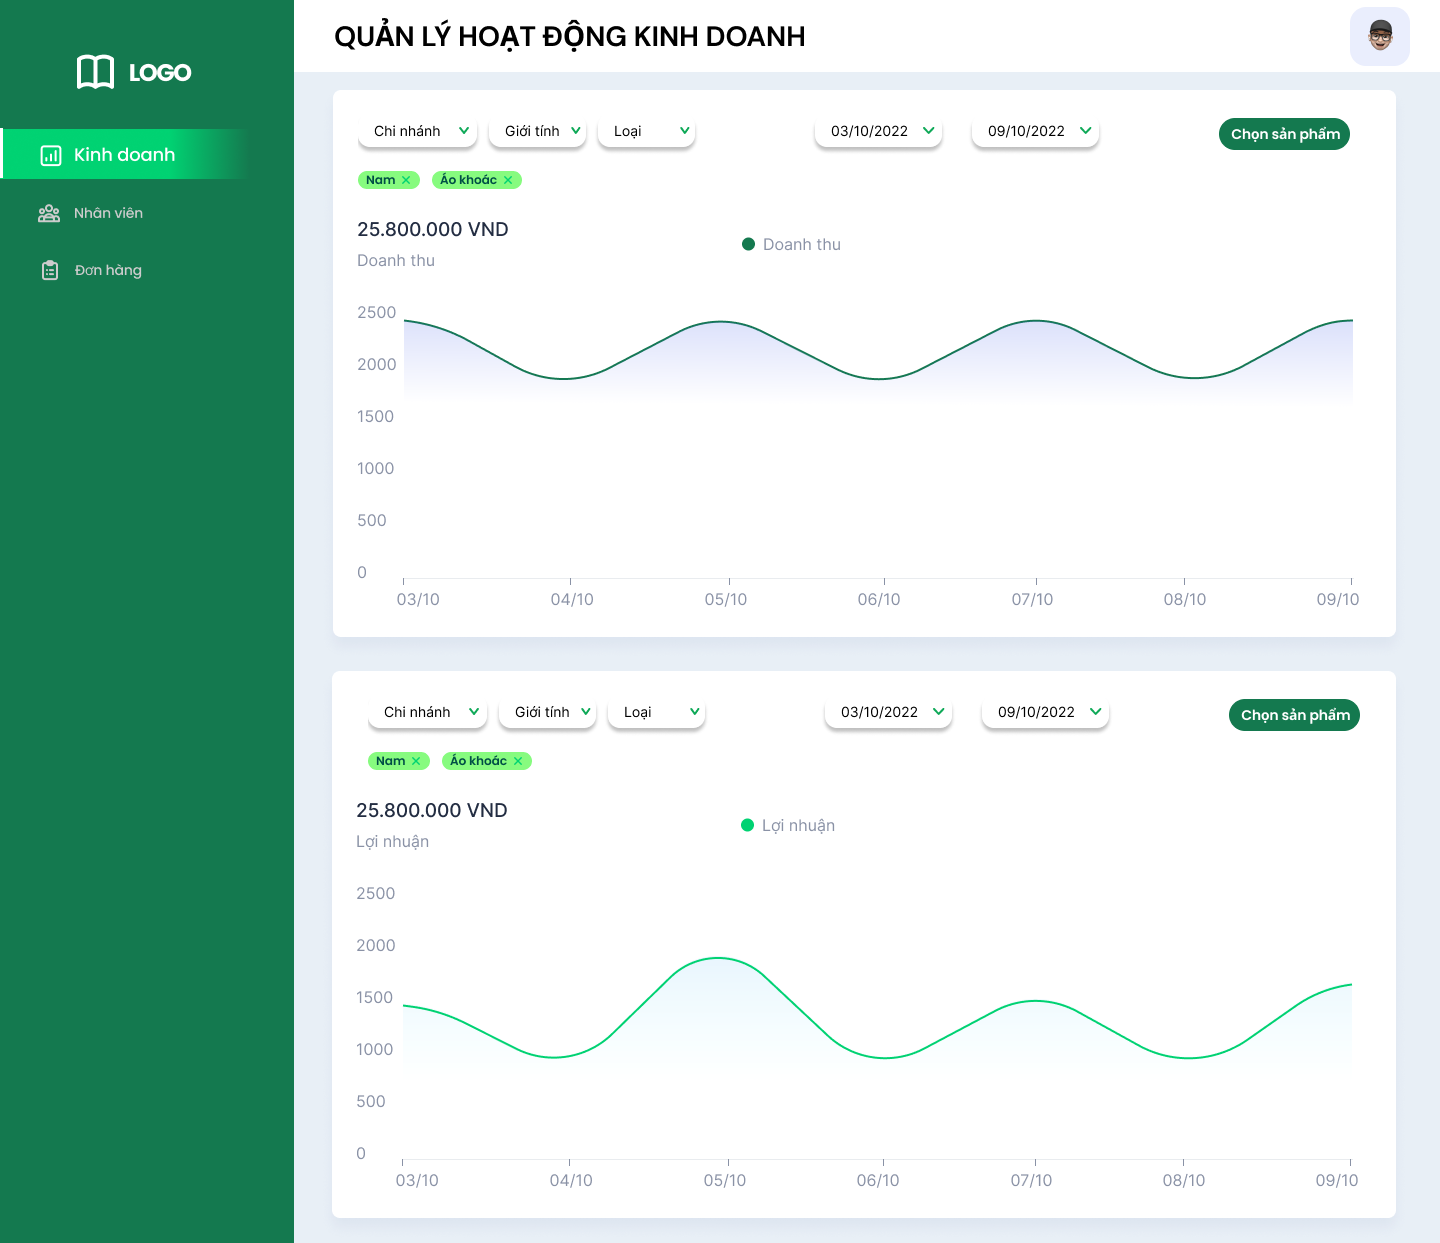
\includegraphics[width=12cm]{img/UI/admin/branch-leader.png}
%     \label{45}
%     \newline
%     \caption{Giao diện của người trưởng chi nhánh}
% \end{figure}
% \newpage


% \subsubsubsection{Quản lý hàng hóa}
% \begin{figure}[!htp]
%     \centering
%     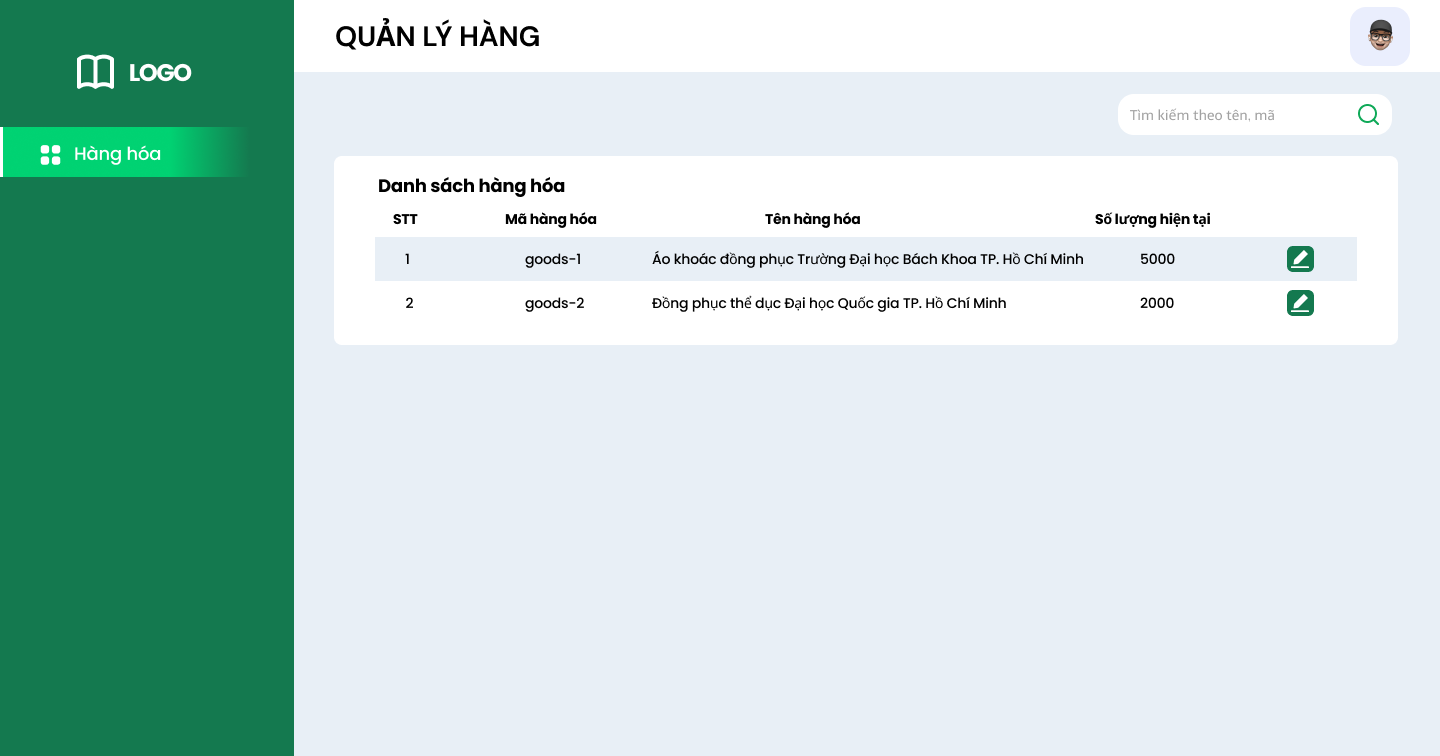
\includegraphics[width=12cm]{img/UI/admin/sub ADmin -Quản lý hàng.png}
%     \label{46}
%     \newline
%     \caption{Giao diện của người quản lý hàng hóa}
% \end{figure}

% \subsubsubsection{Quản lý kho}
% \begin{figure}[!htp]
%     \centering
%     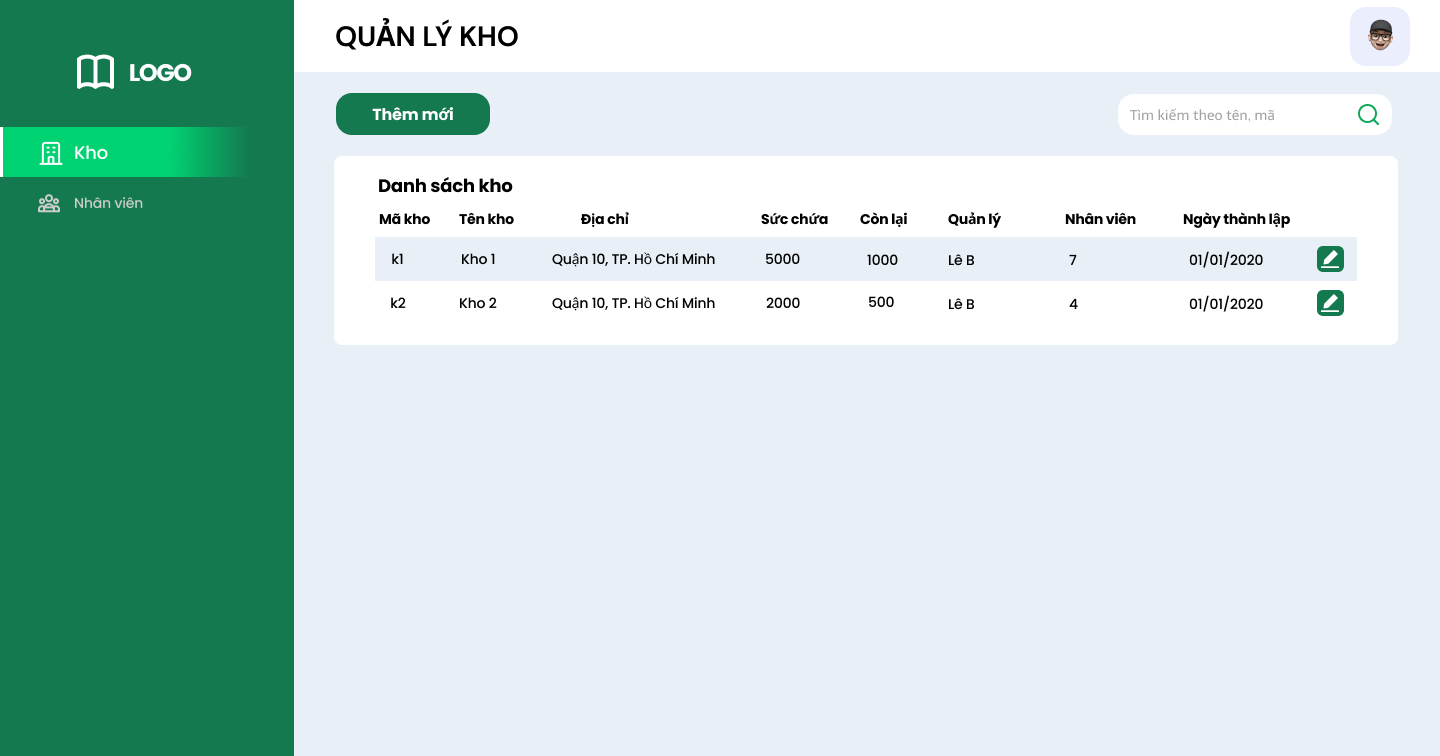
\includegraphics[width=12cm]{img/UI/admin/sub-admin -Quản lý kho.png}
%     \label{47}
%     \newline
%     \caption{Giao diện của người quản lý kho }
% \end{figure}

